\documentclass{article}
\usepackage{graphicx}

\begin{document}
\section*{Problem 1}
    Consider the context-free grammar with $\Sigma = \left\{ a,b \right\}$
    \[S \rightarrow abAB\]
    \[A \rightarrow BC|b|\lambda\]
    \[B \rightarrow BAa|A|a|\lambda\]
    \[C \rightarrow Ab\]

    \begin{enumerate}
        \item Construct a left-most derivation for $abababb$
        \[S \rightarrow abAB \rightarrow abBCB \rightarrow abaCB \rightarrow abaAbB \rightarrow ababB \rightarrow\]
        \[ ababA \rightarrow ababBC \rightarrow ababaC \rightarrow ababaAb \rightarrow abababb\]
        \item Construct the parse tree for your derivation
        \begin{center}
            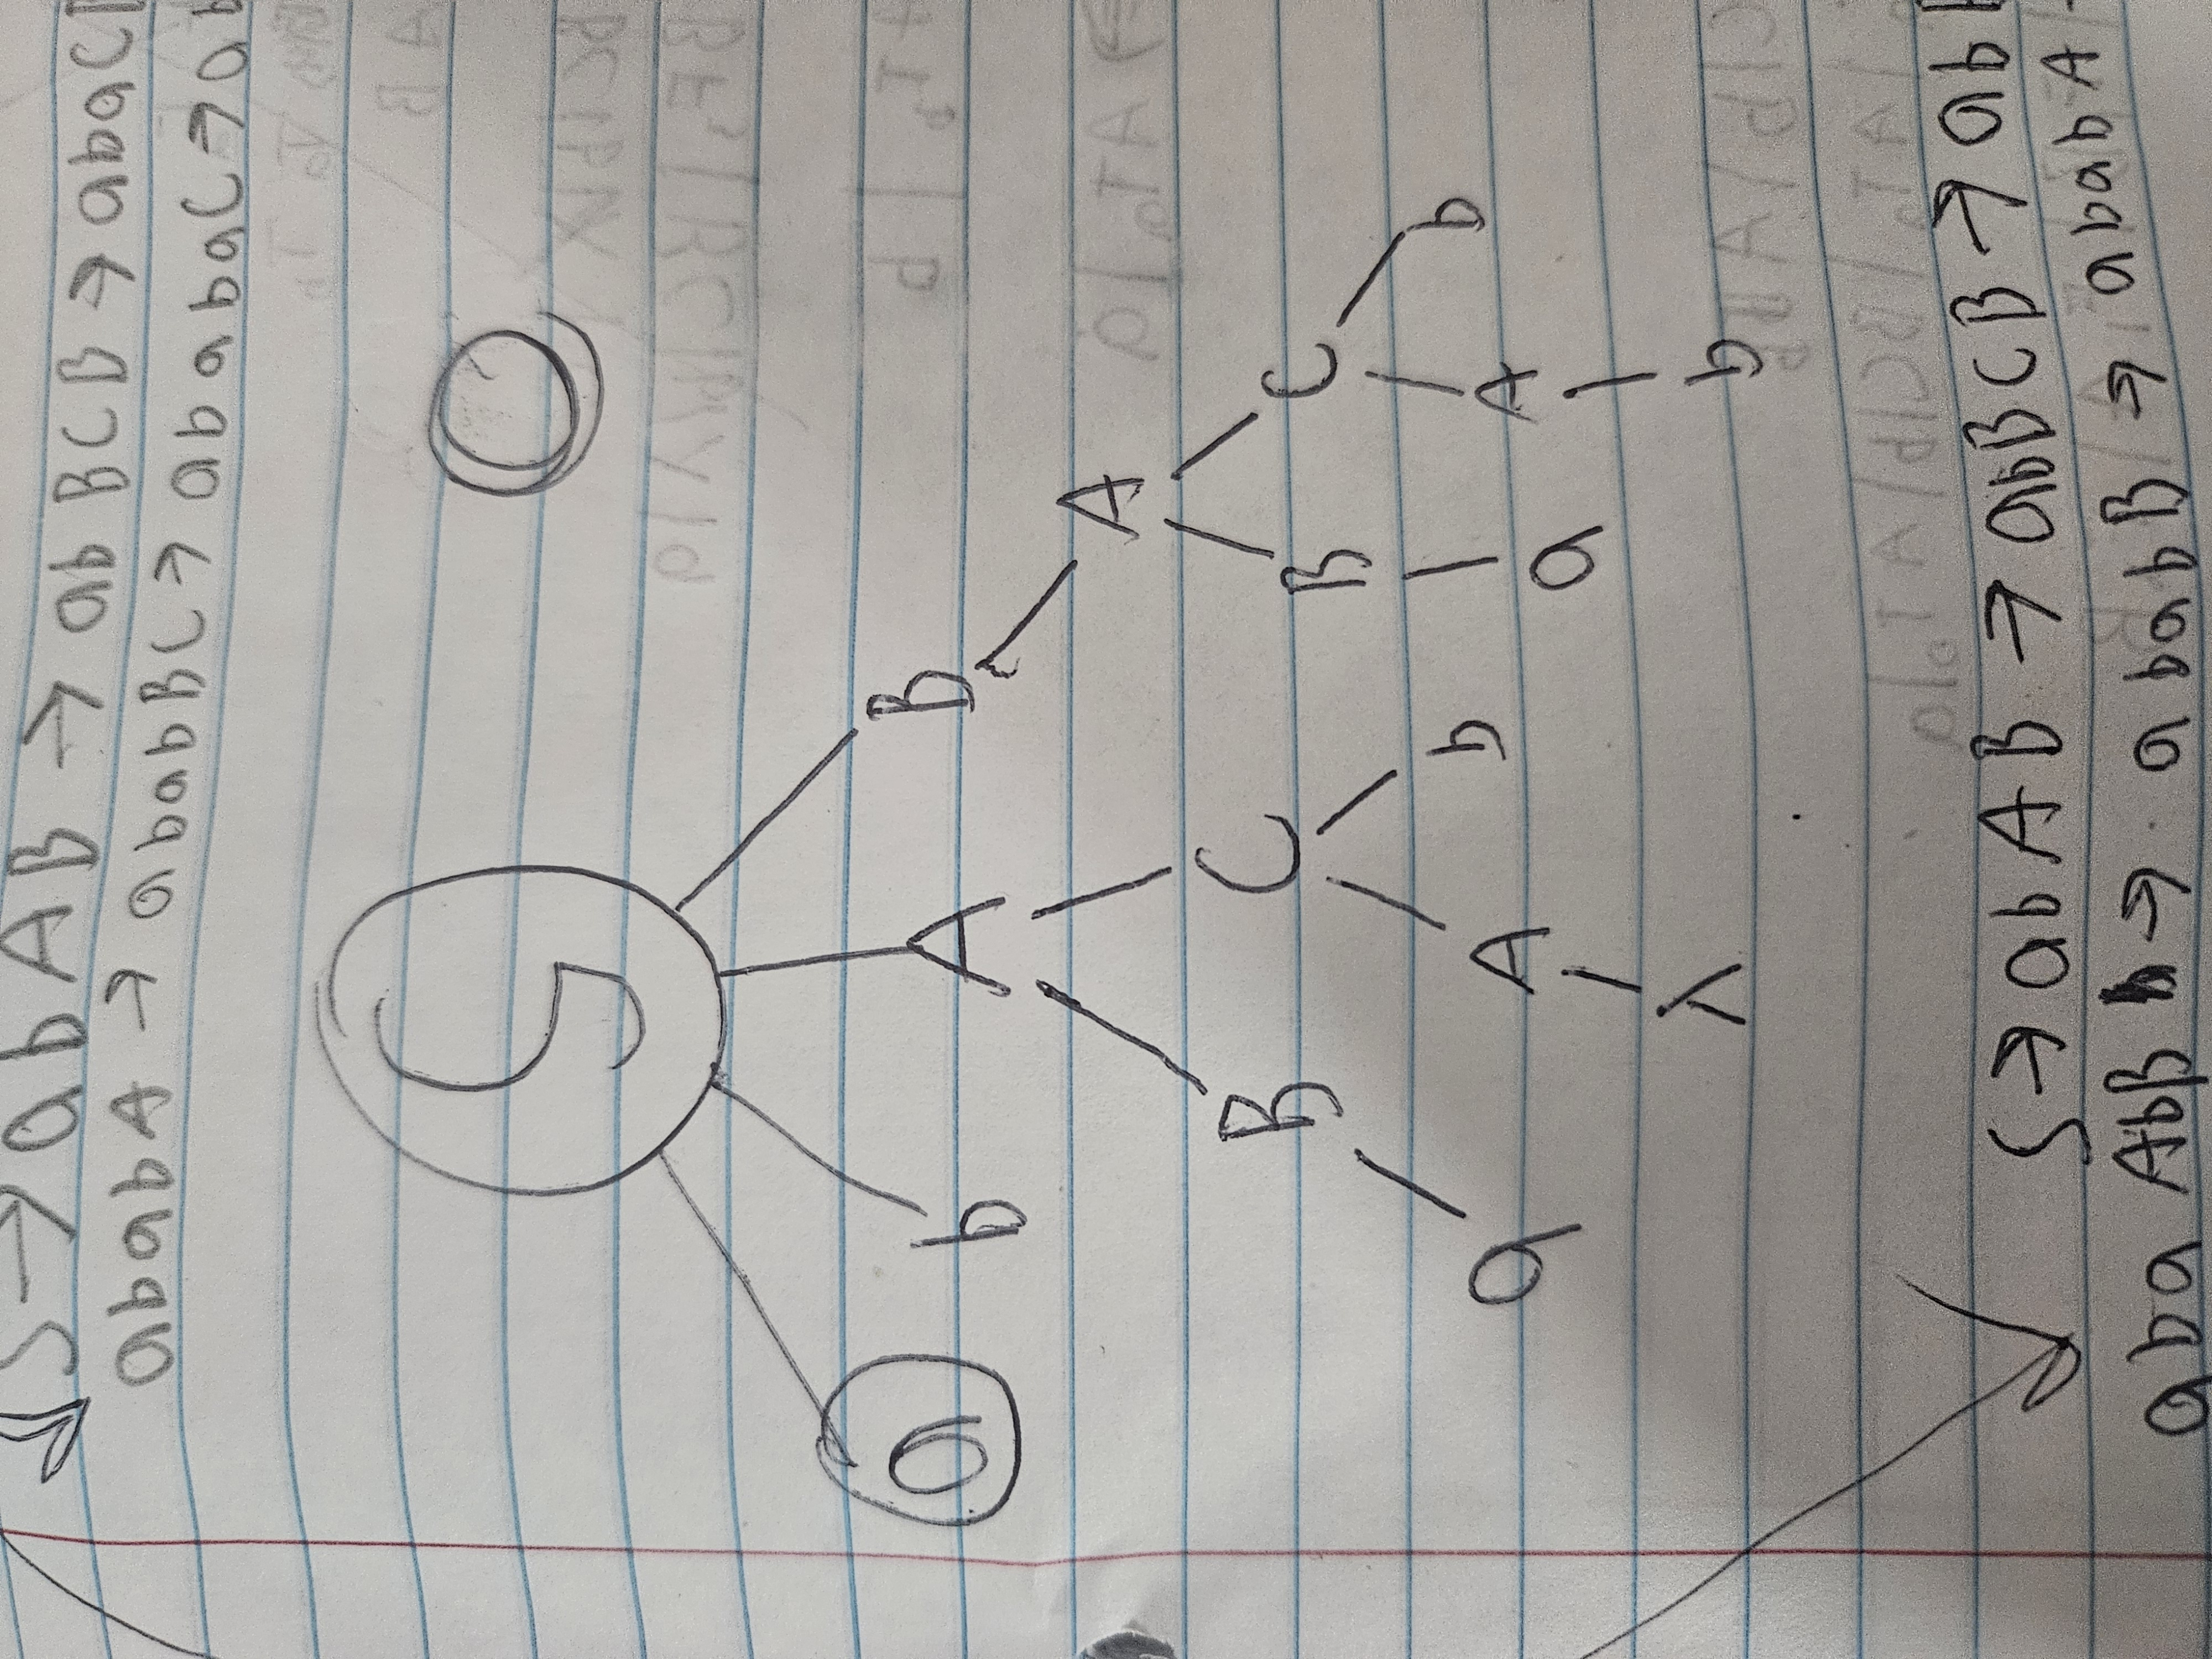
\includegraphics[width=0.5\textwidth, angle=-90]{figures/tree.jpg}
        \end{center}
        \item is L(G) Ambguitous. if so prove item
        yes it is ambiguious as we can derive the follwing left-most derivation
        \[S \rightarrow abAB \rightarrow abBCB \rightarrow abBAaCB \rightarrow abAaCB \rightarrow abaCB \rightarrow abaAbB \rightarrow ababB \rightarrow ababA \rightarrow \]
        \[  ababBC \rightarrow ababC \rightarrow ababAb \rightarrow ababBCb \rightarrow ababaCb \rightarrow ababaAbb \rightarrow abababb\]
        This is clearly a different path yet is a left most derivation thus there is ambiguity  
        \item Convert the grammar to Chomsky Normal Form.
        \newpage
        Here is the following cooresponding Chomsky Normal form
        \[T_a \rightarrow a\]
        \[T_b \rightarrow b\]
        \[A \rightarrow BC | b | AT_b\]
        \[ B \rightarrow BT_a | A T_a | BC | AT_b | a\]
        \[S \rightarrow T_aT_b | F_1 B | F_1 A | F_2 B\]
        \[F_1 \rightarrow T_a T_b\]
        \[F_2 \rightarrow F_1A\]
    \end{enumerate}
    \section*{Problem 2}
    Find a context free grammar and draw a push down automata for $L = \left\{ a^nb^n: n\ge 0\right\}$ 
    Show the sequence of instanteous description for $aaaabbbb$
    $\\$
    Heres the context free grammar
    \[ S \rightarrow aSb | \lambda\]

    Here is the following Push Down Automata Diagram
    \begin{center}
        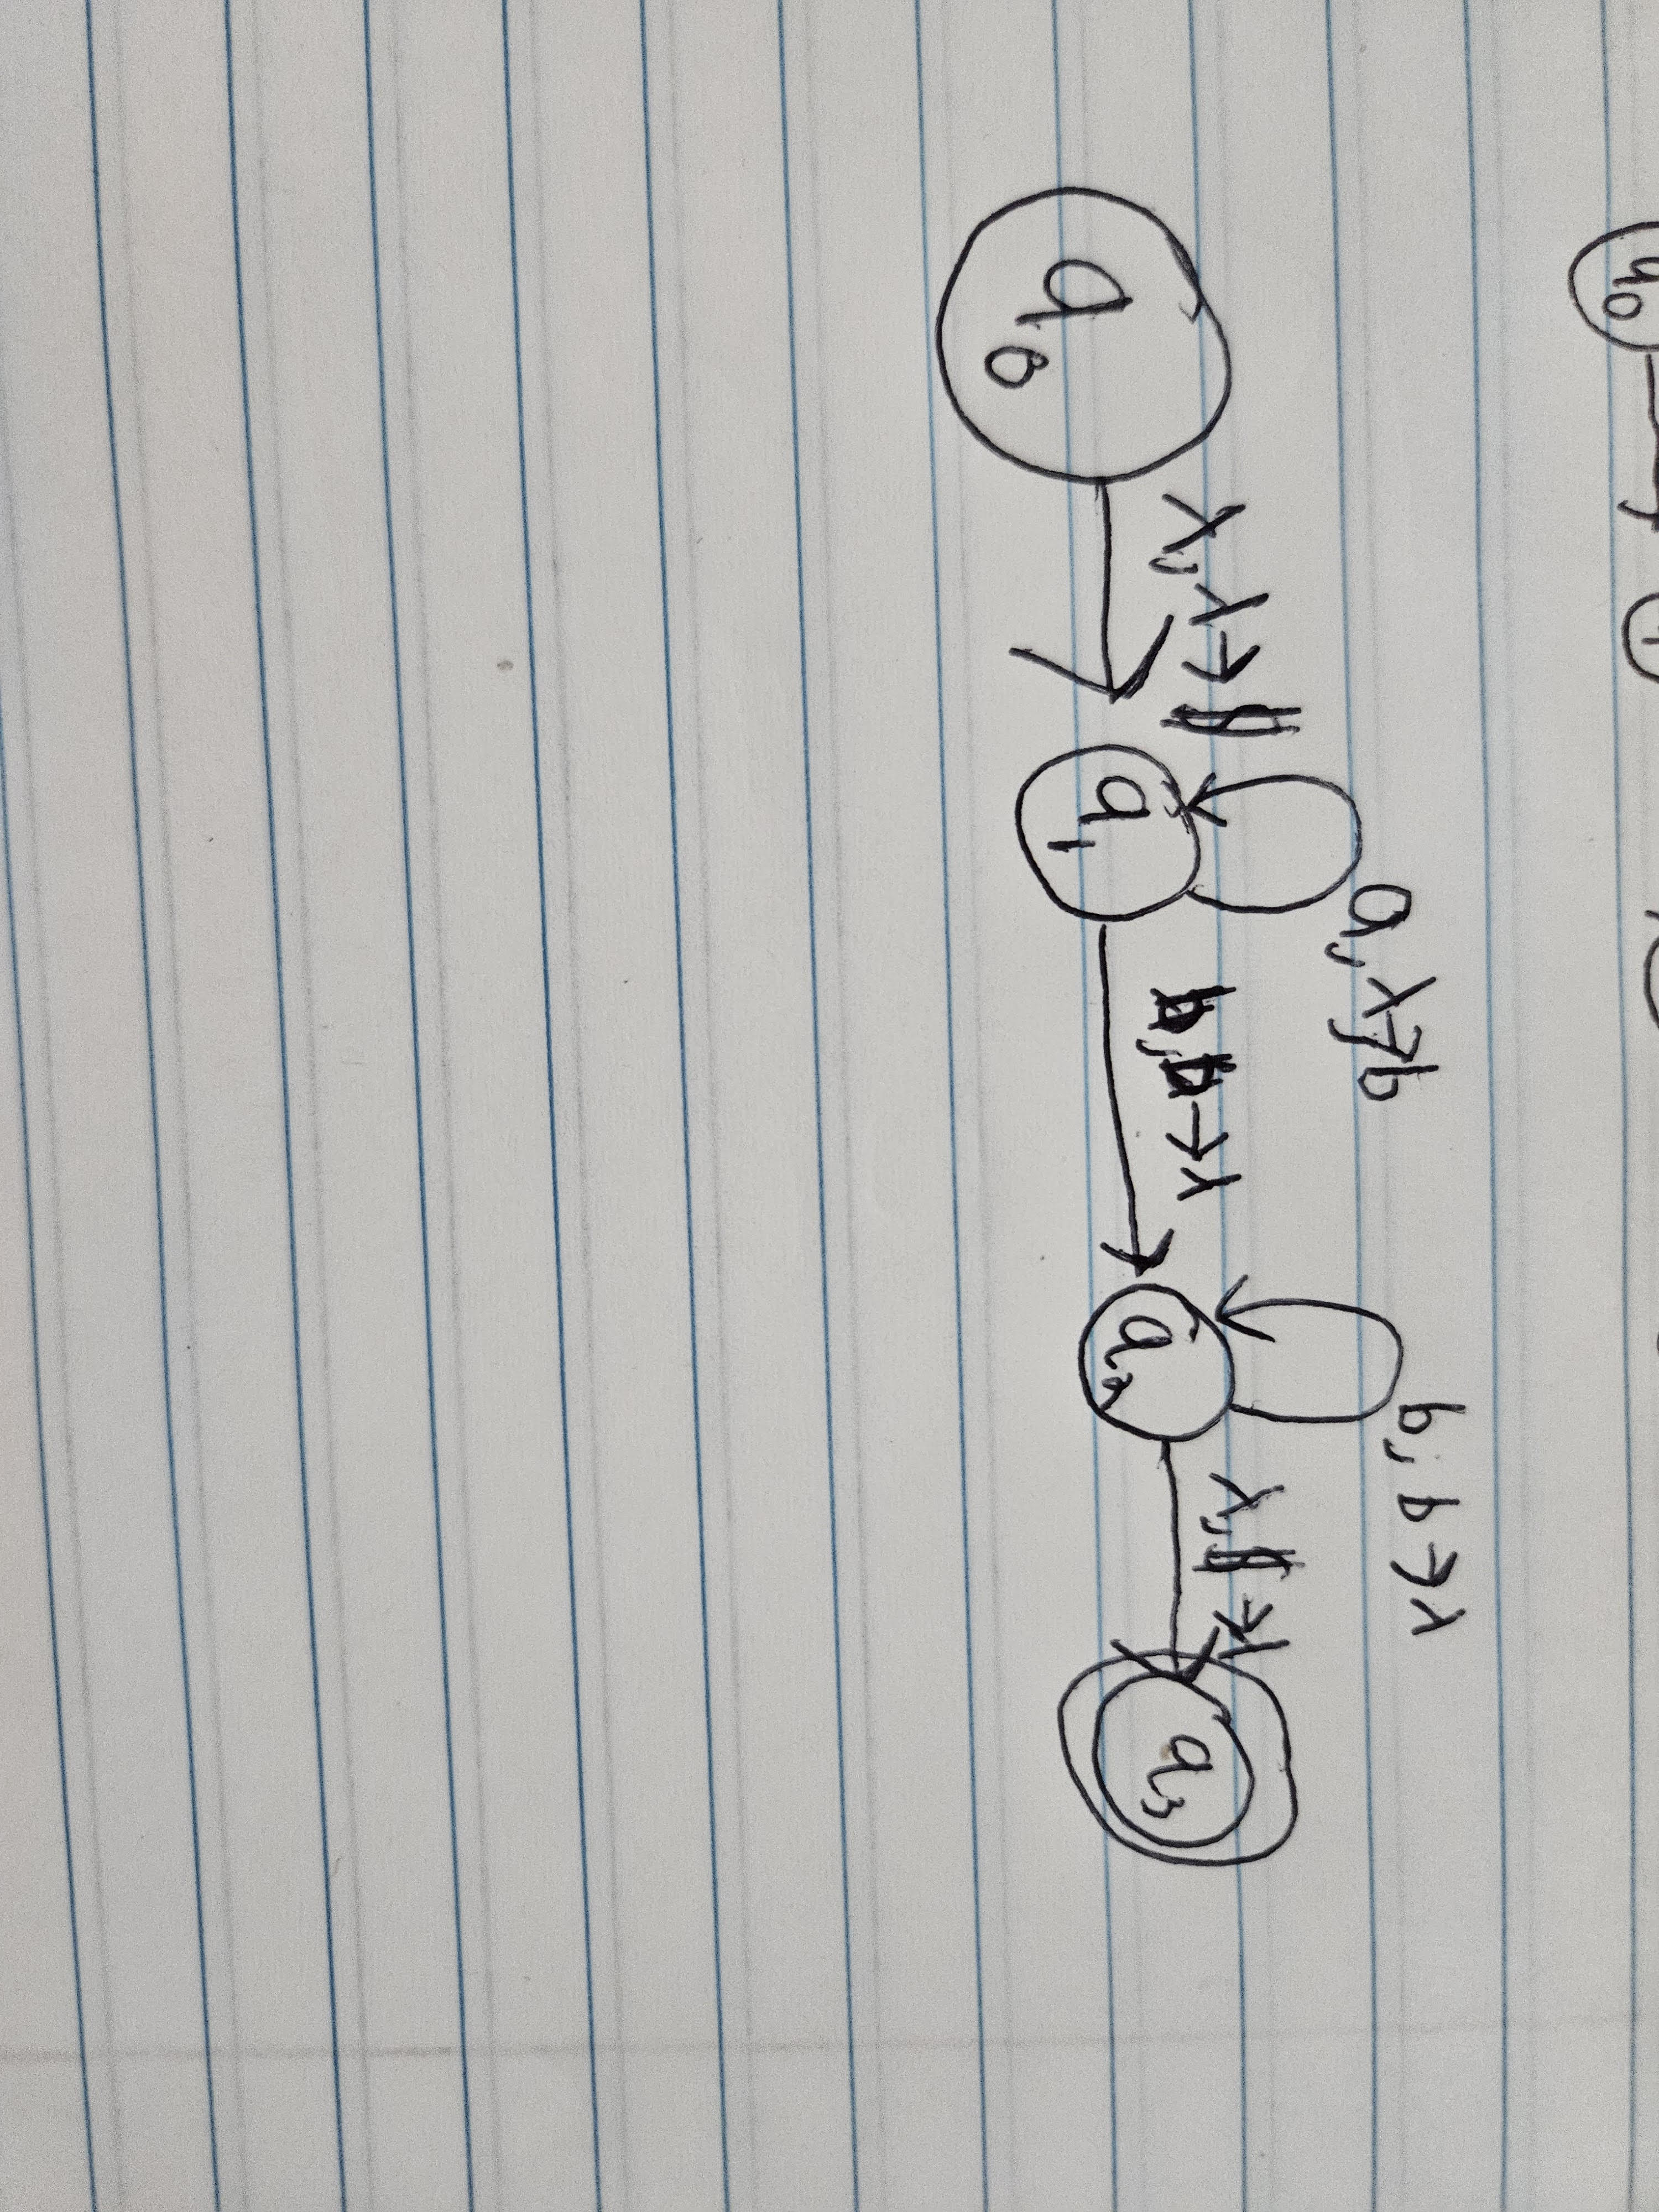
\includegraphics[width=0.5\textwidth, angle=90]{figures/figures_PDA1.jpg}
    \end{center}

    \newpage
    The instanteous description for $aaaabbbb$ is 

    \[\left(q_0, aaaabbbb, \lambda\right)\]
    \[\left(q_1, aaaabbbb, \$\right)\]
    \[\left(q_1, aaabbbb, b\$\right)\]
    \[\left(q_1, aabbbb, bb\$\right)\]
    \[\left(q_1, abbbb, bbb\$\right)\]
    \[\left(q_1, bbbb, bbbb\$\right)\]
    \[\left(q_2, bbbb, bbbb\$\right)\]
    \[\left(q_2, bbb, bbb\$\right)\]
    \[\left(q_2, bb, bb\$\right)\]
    \[\left(q_2, b, b\$\right)\]
    \[\left(q_2, \lambda, \$\right)\]
    \[\left(q_3, \lambda, \lambda\right)\]


    \section*{Problem 3}
    Find the Context Free Grammar and Push Down Automate Diagram for \[L = \left\{ ww^R|w \in \left\{a,b \right\} ^* \right\} \] and give the instanteous description for $bbaabb \\$

    Here is the following Context Free Grammar
    \[S \rightarrow aSa | bSb | \lambda\]
    \newpage
    Here is the PDA Diagram
    \begin{center}
        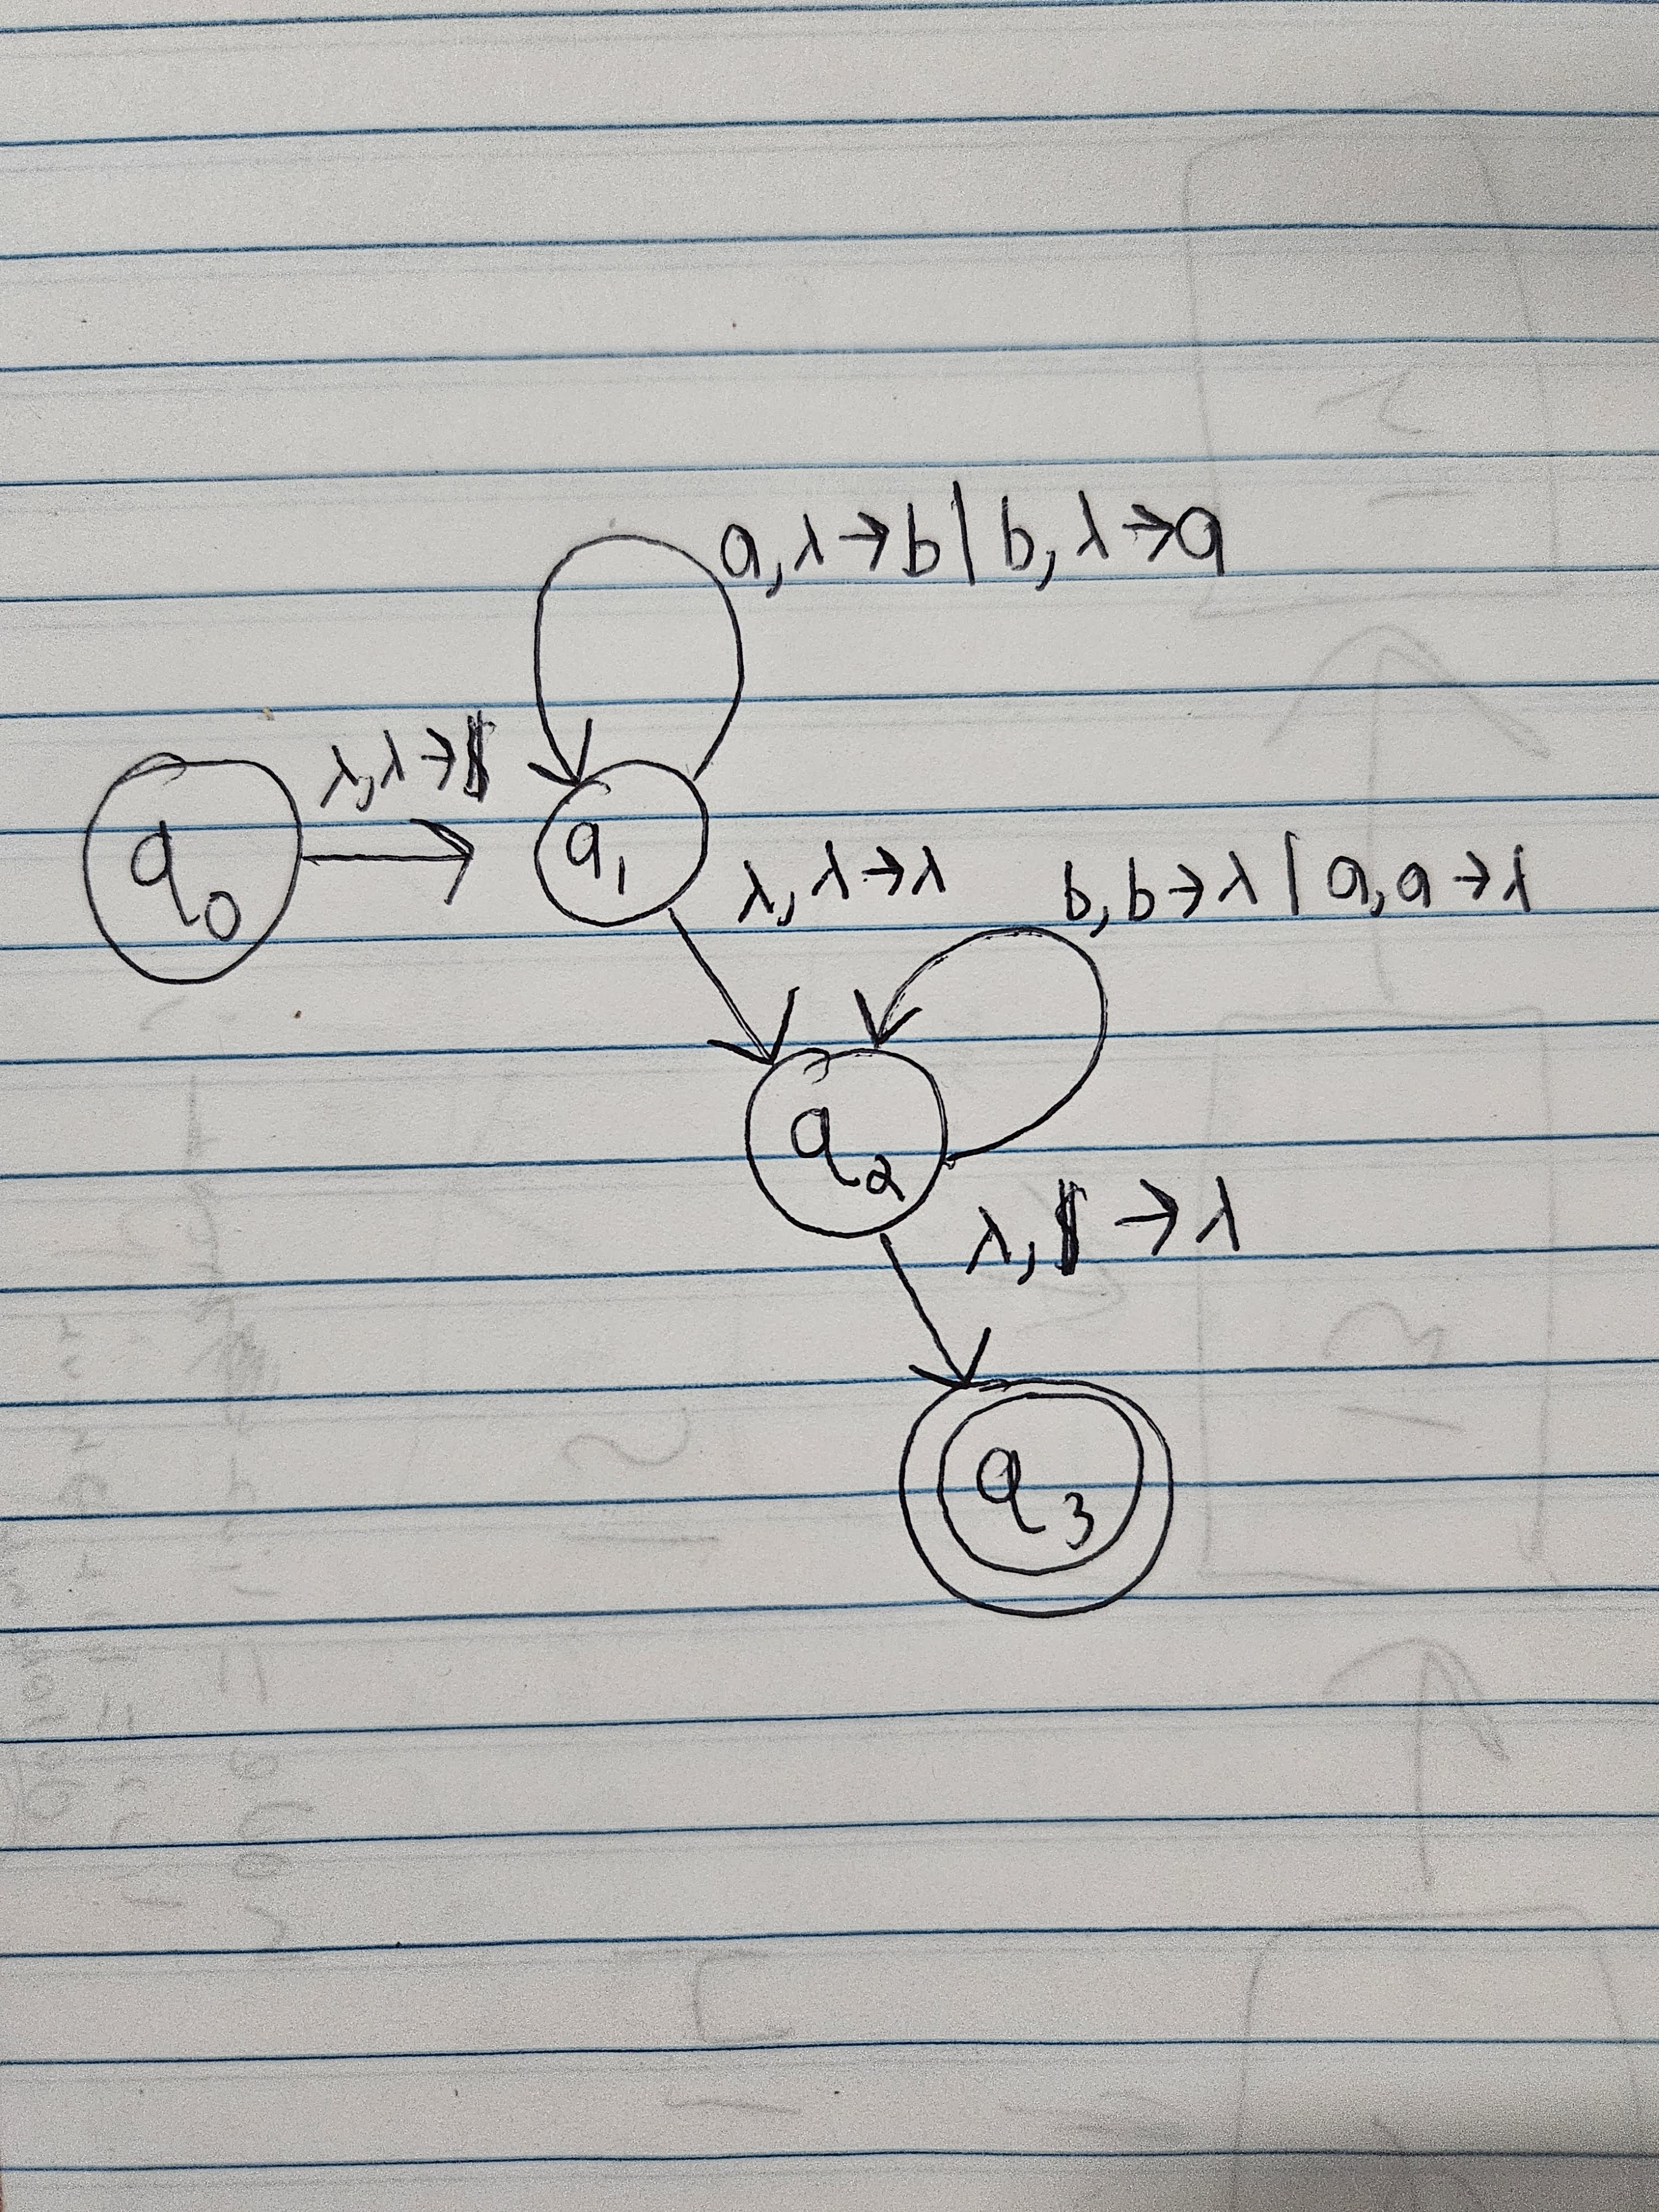
\includegraphics[width=0.5\textwidth]{figures/figures_PDA2.jpg}
    \end{center}
    Lastly, here is the instanteous description for $bbaabb$
    \[\left(q_0, bbaabb, \lambda\right)\]
    \[\left(q_1, bbaabb, \$\right)\]
    \[\left(q_1, baabb, b\$\right)\]
    \[\left(q_1, aabb, bb\$\right)\]
    \[\left(q_1, abb, abb\$\right)\]
    \[\left(q_2, abb, abb\$\right)\]
    \[\left(q_2, bb, bb\$\right)\]
    \[\left(q_2, b, b\$\right)\]
    \[\left(q_2, \lambda, \$\right)\]
    \[\left(q_3, \lambda, \lambda\right)\]

    \newpage
    \section*{Problem 4}
    Find the Context Free Grammar and Push Down Automata Diagram for \[\left\{ w \in \left\{ a,b\right\}* : n_a\left(w\right) n_b\left(w\right) \right\}\]
    Then give the instanteous description of $bbaaab\\\\$
    Here is the context grammar
    \[S \rightarrow \lambda | Sab | aSb | abS | Sba | bSa | baS\]
    $\\$
    Here is the PDA Diagram
    \begin{center}
        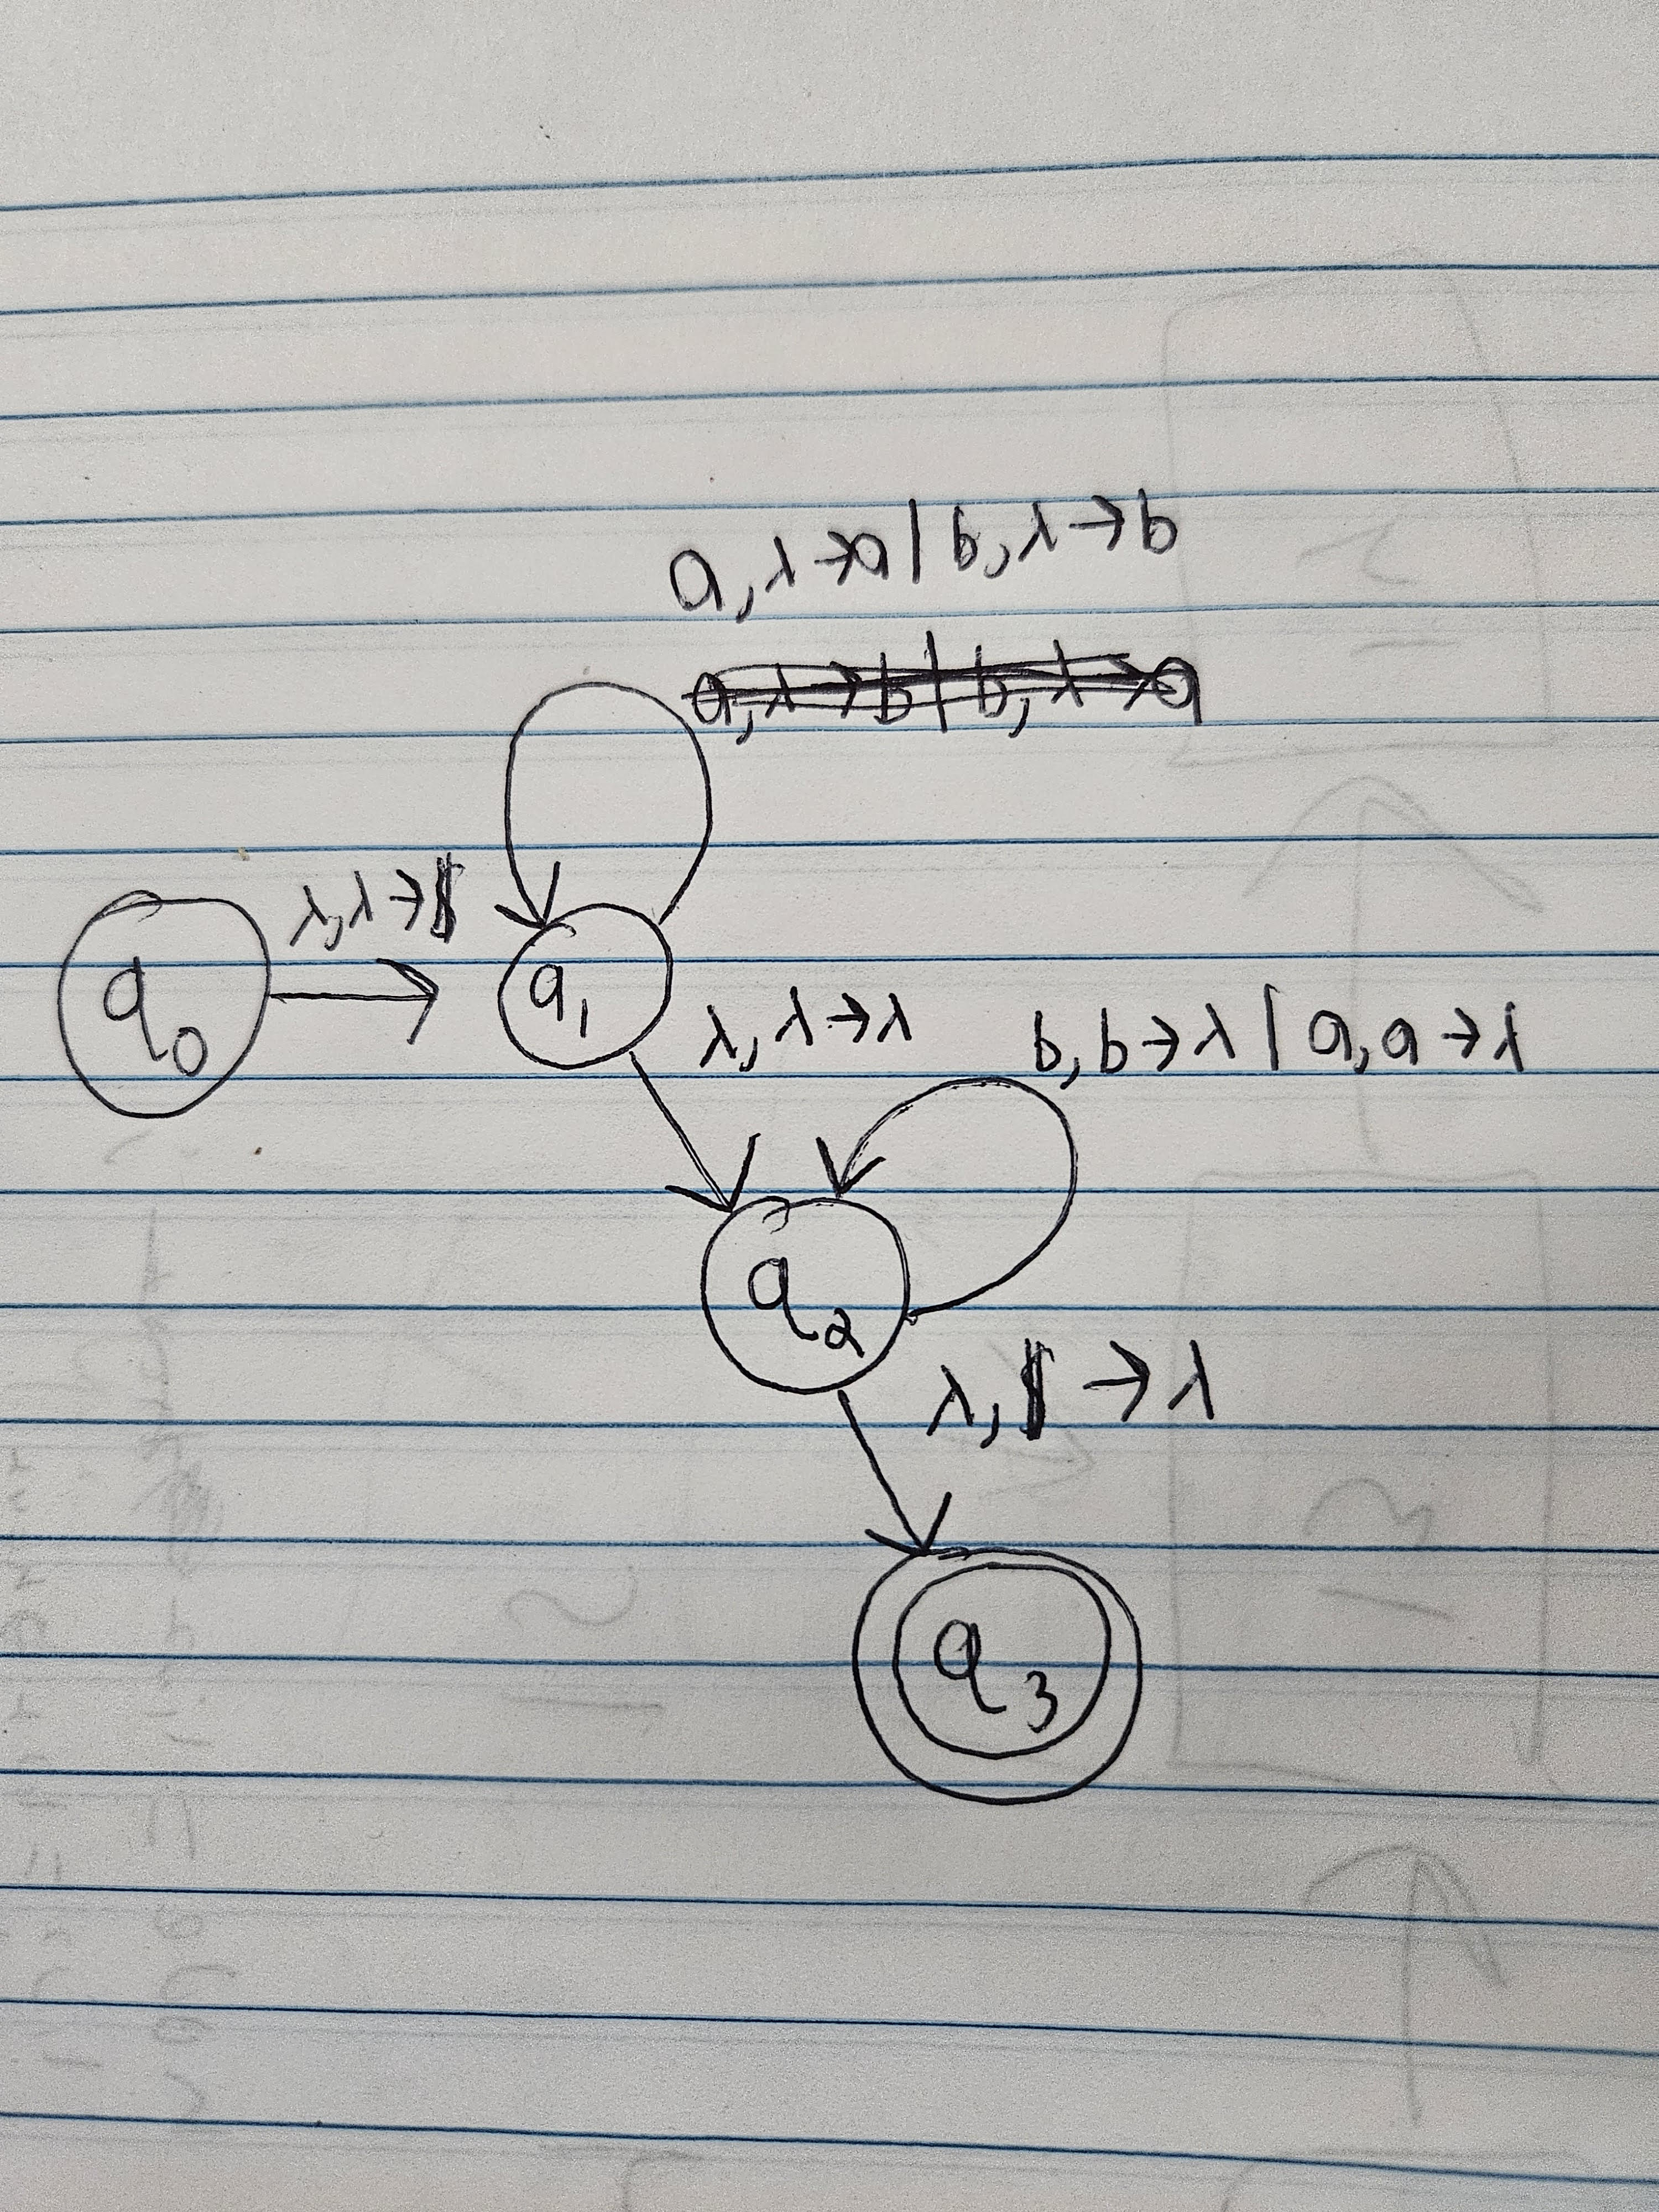
\includegraphics[width=0.5\textwidth]{figures/figures_PDA3.jpg}
    \end{center}

    Here is the instanteous description for $bbaaab\\$
    \[\left(q_0, bbaaab, \lambda\right)\]
    \[\left(q_1, bbaaab, \$ \right)\]
    \[\left(q_1, baaab, a\$ \right)\]
    \[\left(q_1, aaab, aa\$ \right)\]
    \[\left(q_1, aab, a\$ \right)\]
    \[\left(q_1, ab, \$ \right)\]
    \[\left(q_1, b, b\$ \right)\]
    \[\left(q_1, \lambda, \$ \right)\]
    \[\left(q_2, \lambda, \lambda \right)\]

    \section*{Question 2}
    \begin{enumerate}
        \item With the given production rules we have the following LR Parsings
        \[ S' \rightarrow \cdot{} S\]
        \[ S' \rightarrow \cdot{} Sa\]
        \[ S' \rightarrow \cdot{} bA\]
        \item What are the outgoing transistions from initial state and their labels 
		There exists 2 outgoing transistions S, b
	\item Construct the DFA Diagram for this Grammar
	\begin{center}
            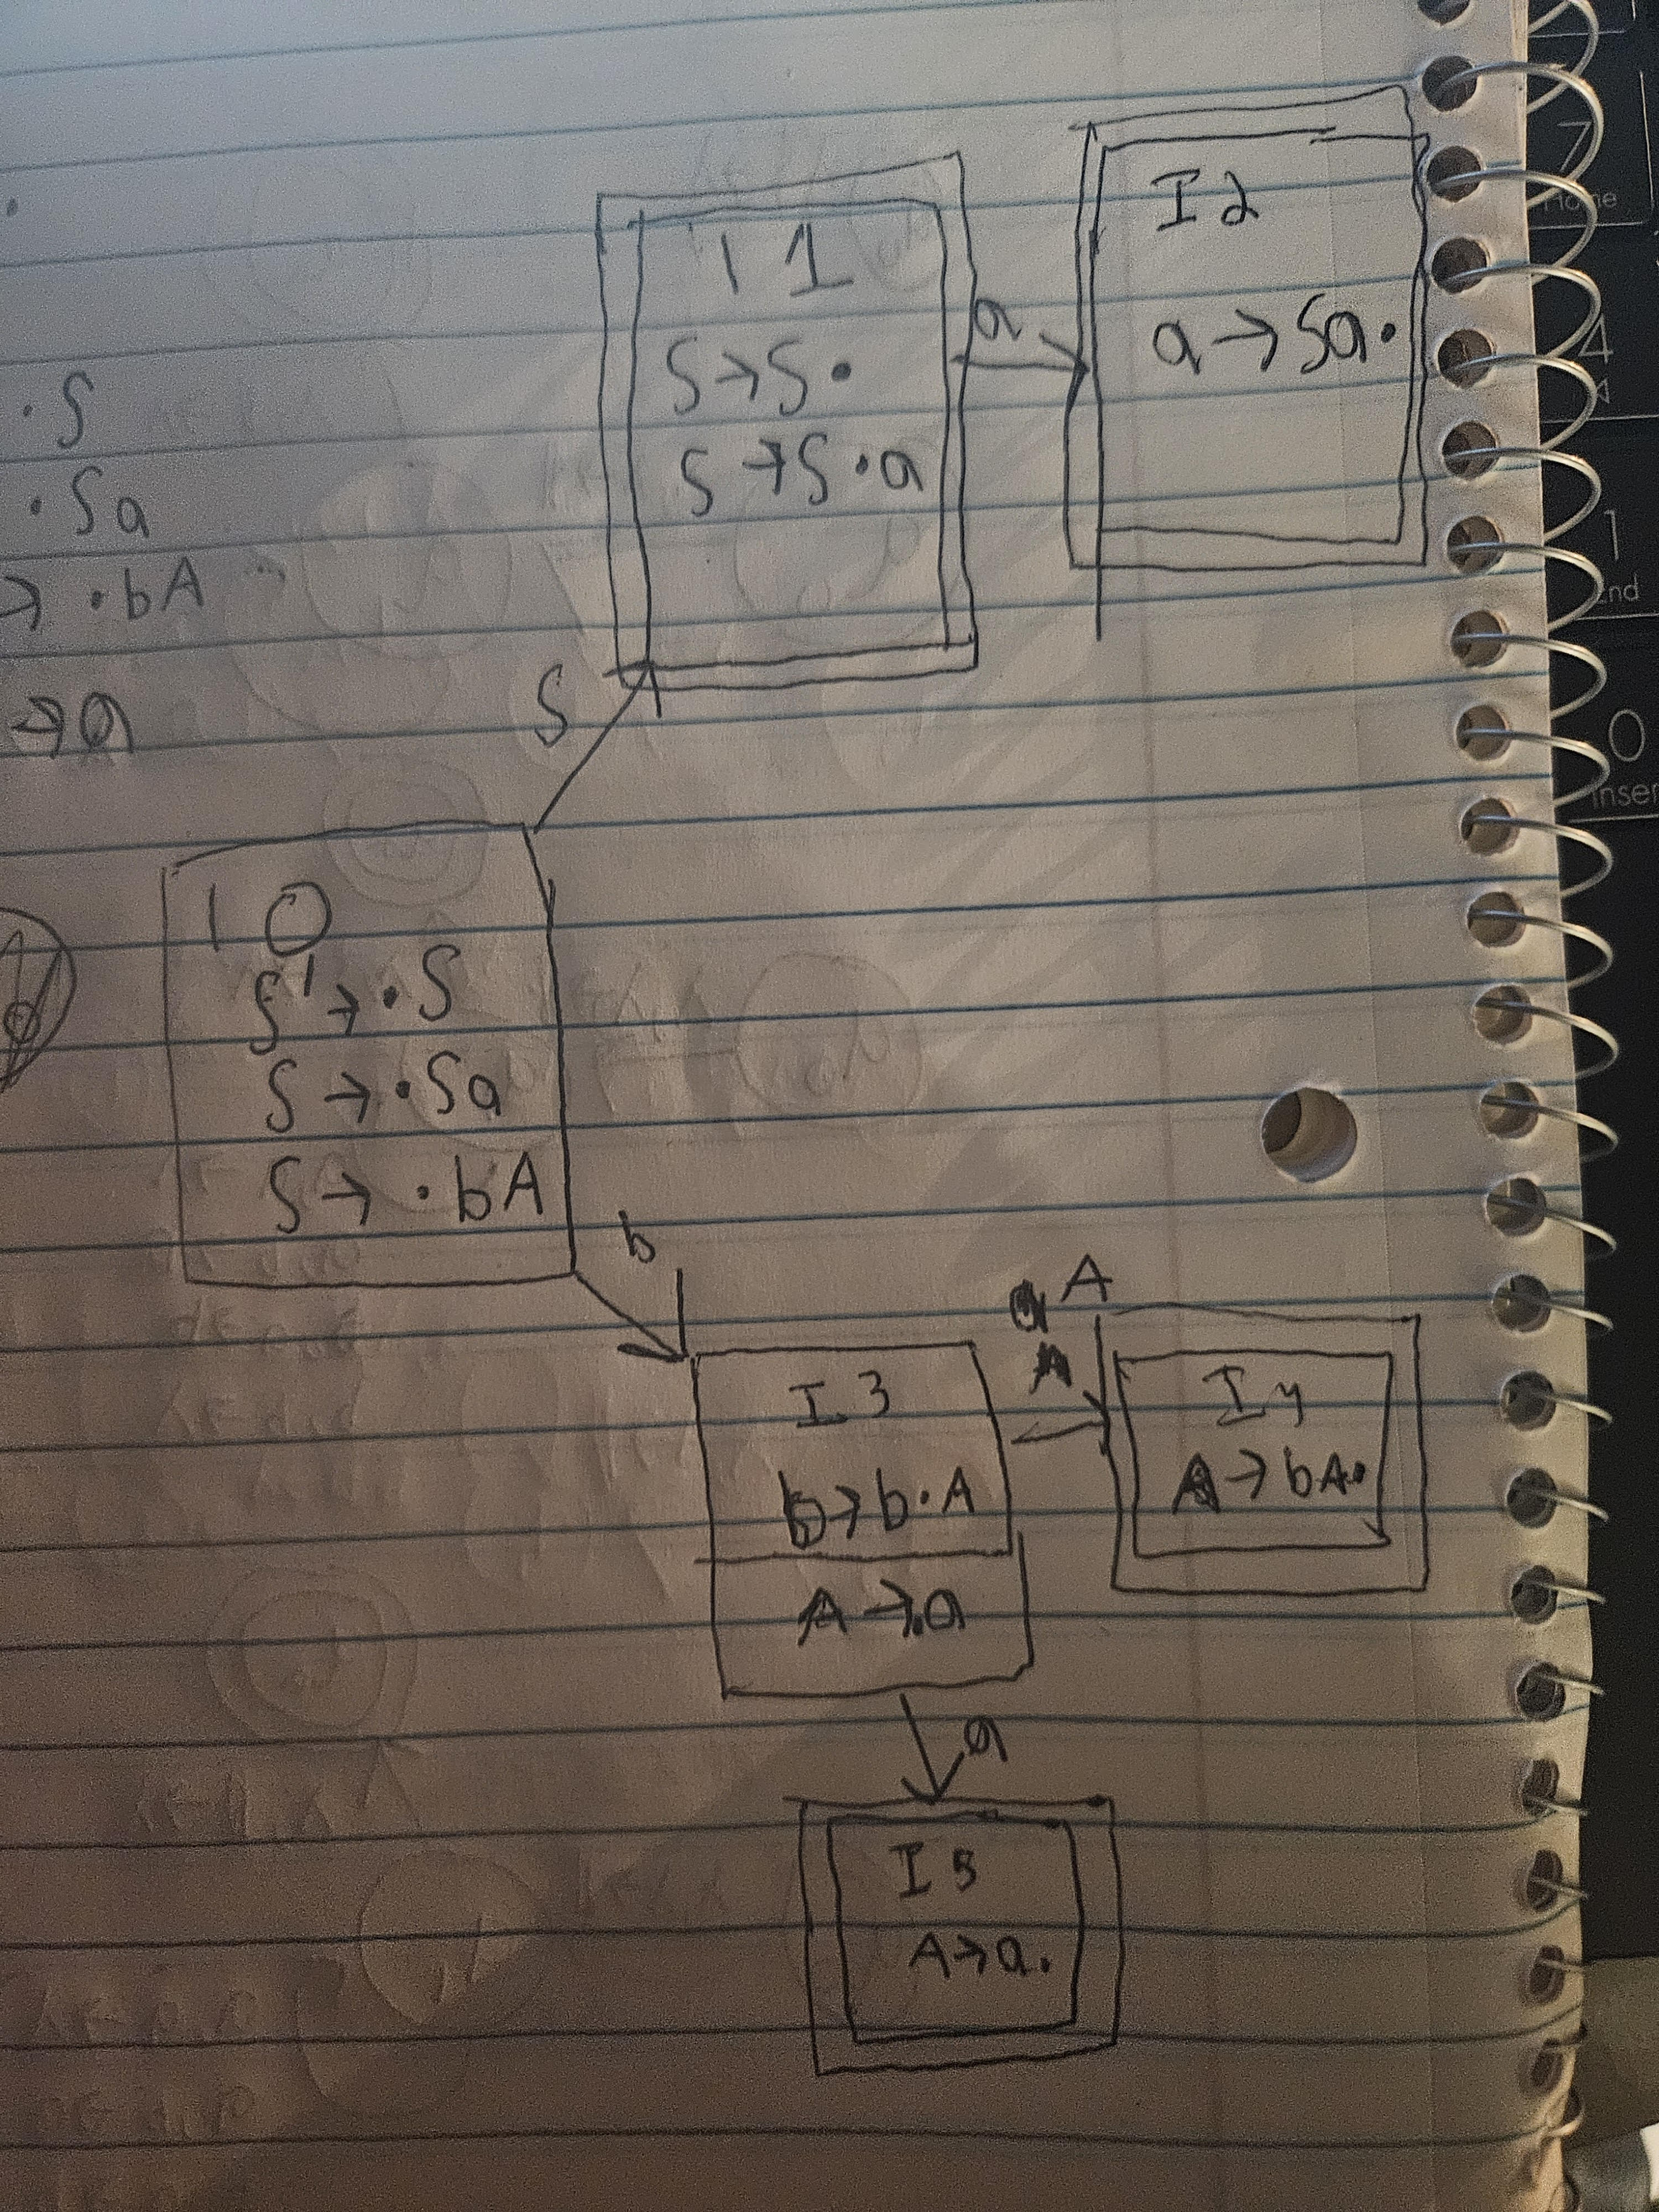
\includegraphics[width=0.5\textwidth, angle=0]{figures/DFA1.jpg}
	\end{center}
    	\end{enumerate}

    \section*{Question 3}
    \begin{enumerate}
	\item give the item set for the closure $S' \rightarrow S$
		\[ S' \rightarrow \cdot{} S\]
		\[ S \rightarrow \cdot{} aS\]
		\[ S \rightarrow \cdot{} cA\]
	\item Give the number of outgoing transitions
	There exists 3 labels the following S, a, c
	\item Construct the DFA
	\begin{center}
            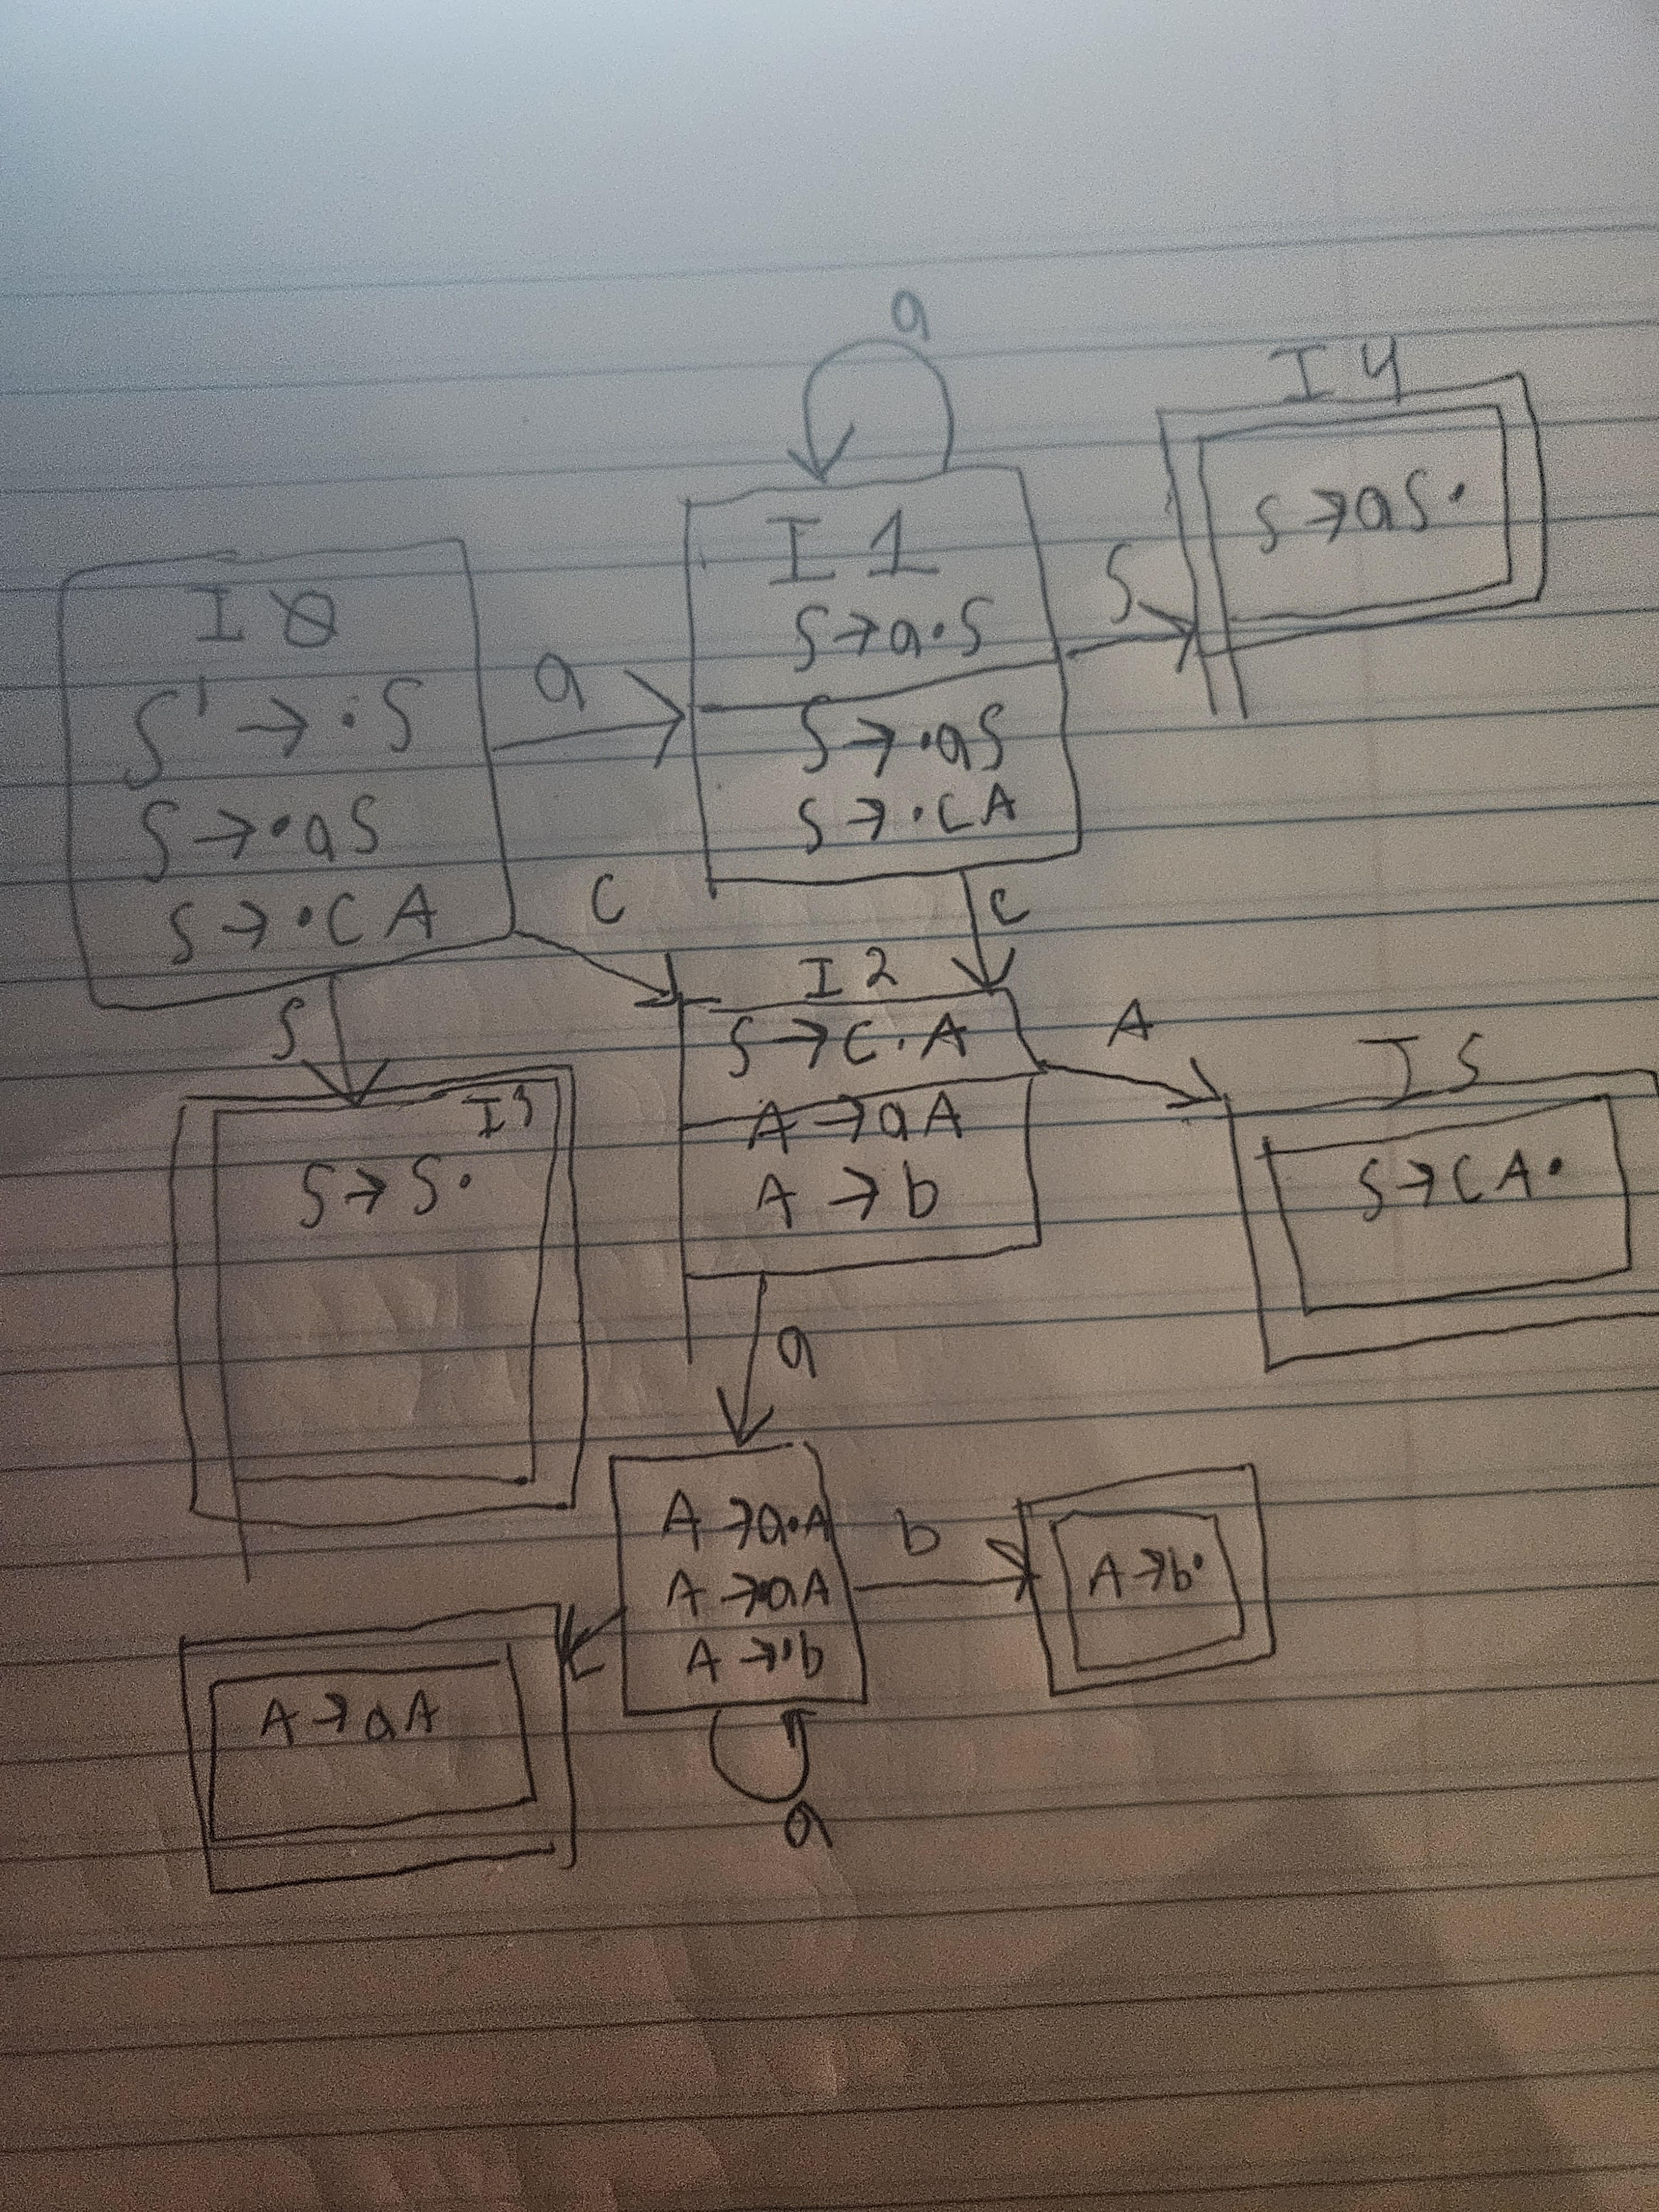
\includegraphics[width=0.5\textwidth, angle=0]{figures/DFA2.jpg}
	\end{center}
    \end{enumerate}

\newpage
    \section*{Question 4}
    \begin{enumerate}
	\item Give the initial item set
		\[S' \rightarrow S\]
		\[S \rightarrow bbS\]
		\[S \rightarrow aAa\]
	\item How many Initial Outgoing states are there and What are there labels
	There exists 3 labels that are coming out of S' they are S, b, a
	\item Give complete DFA Diagram
	\begin{center}
            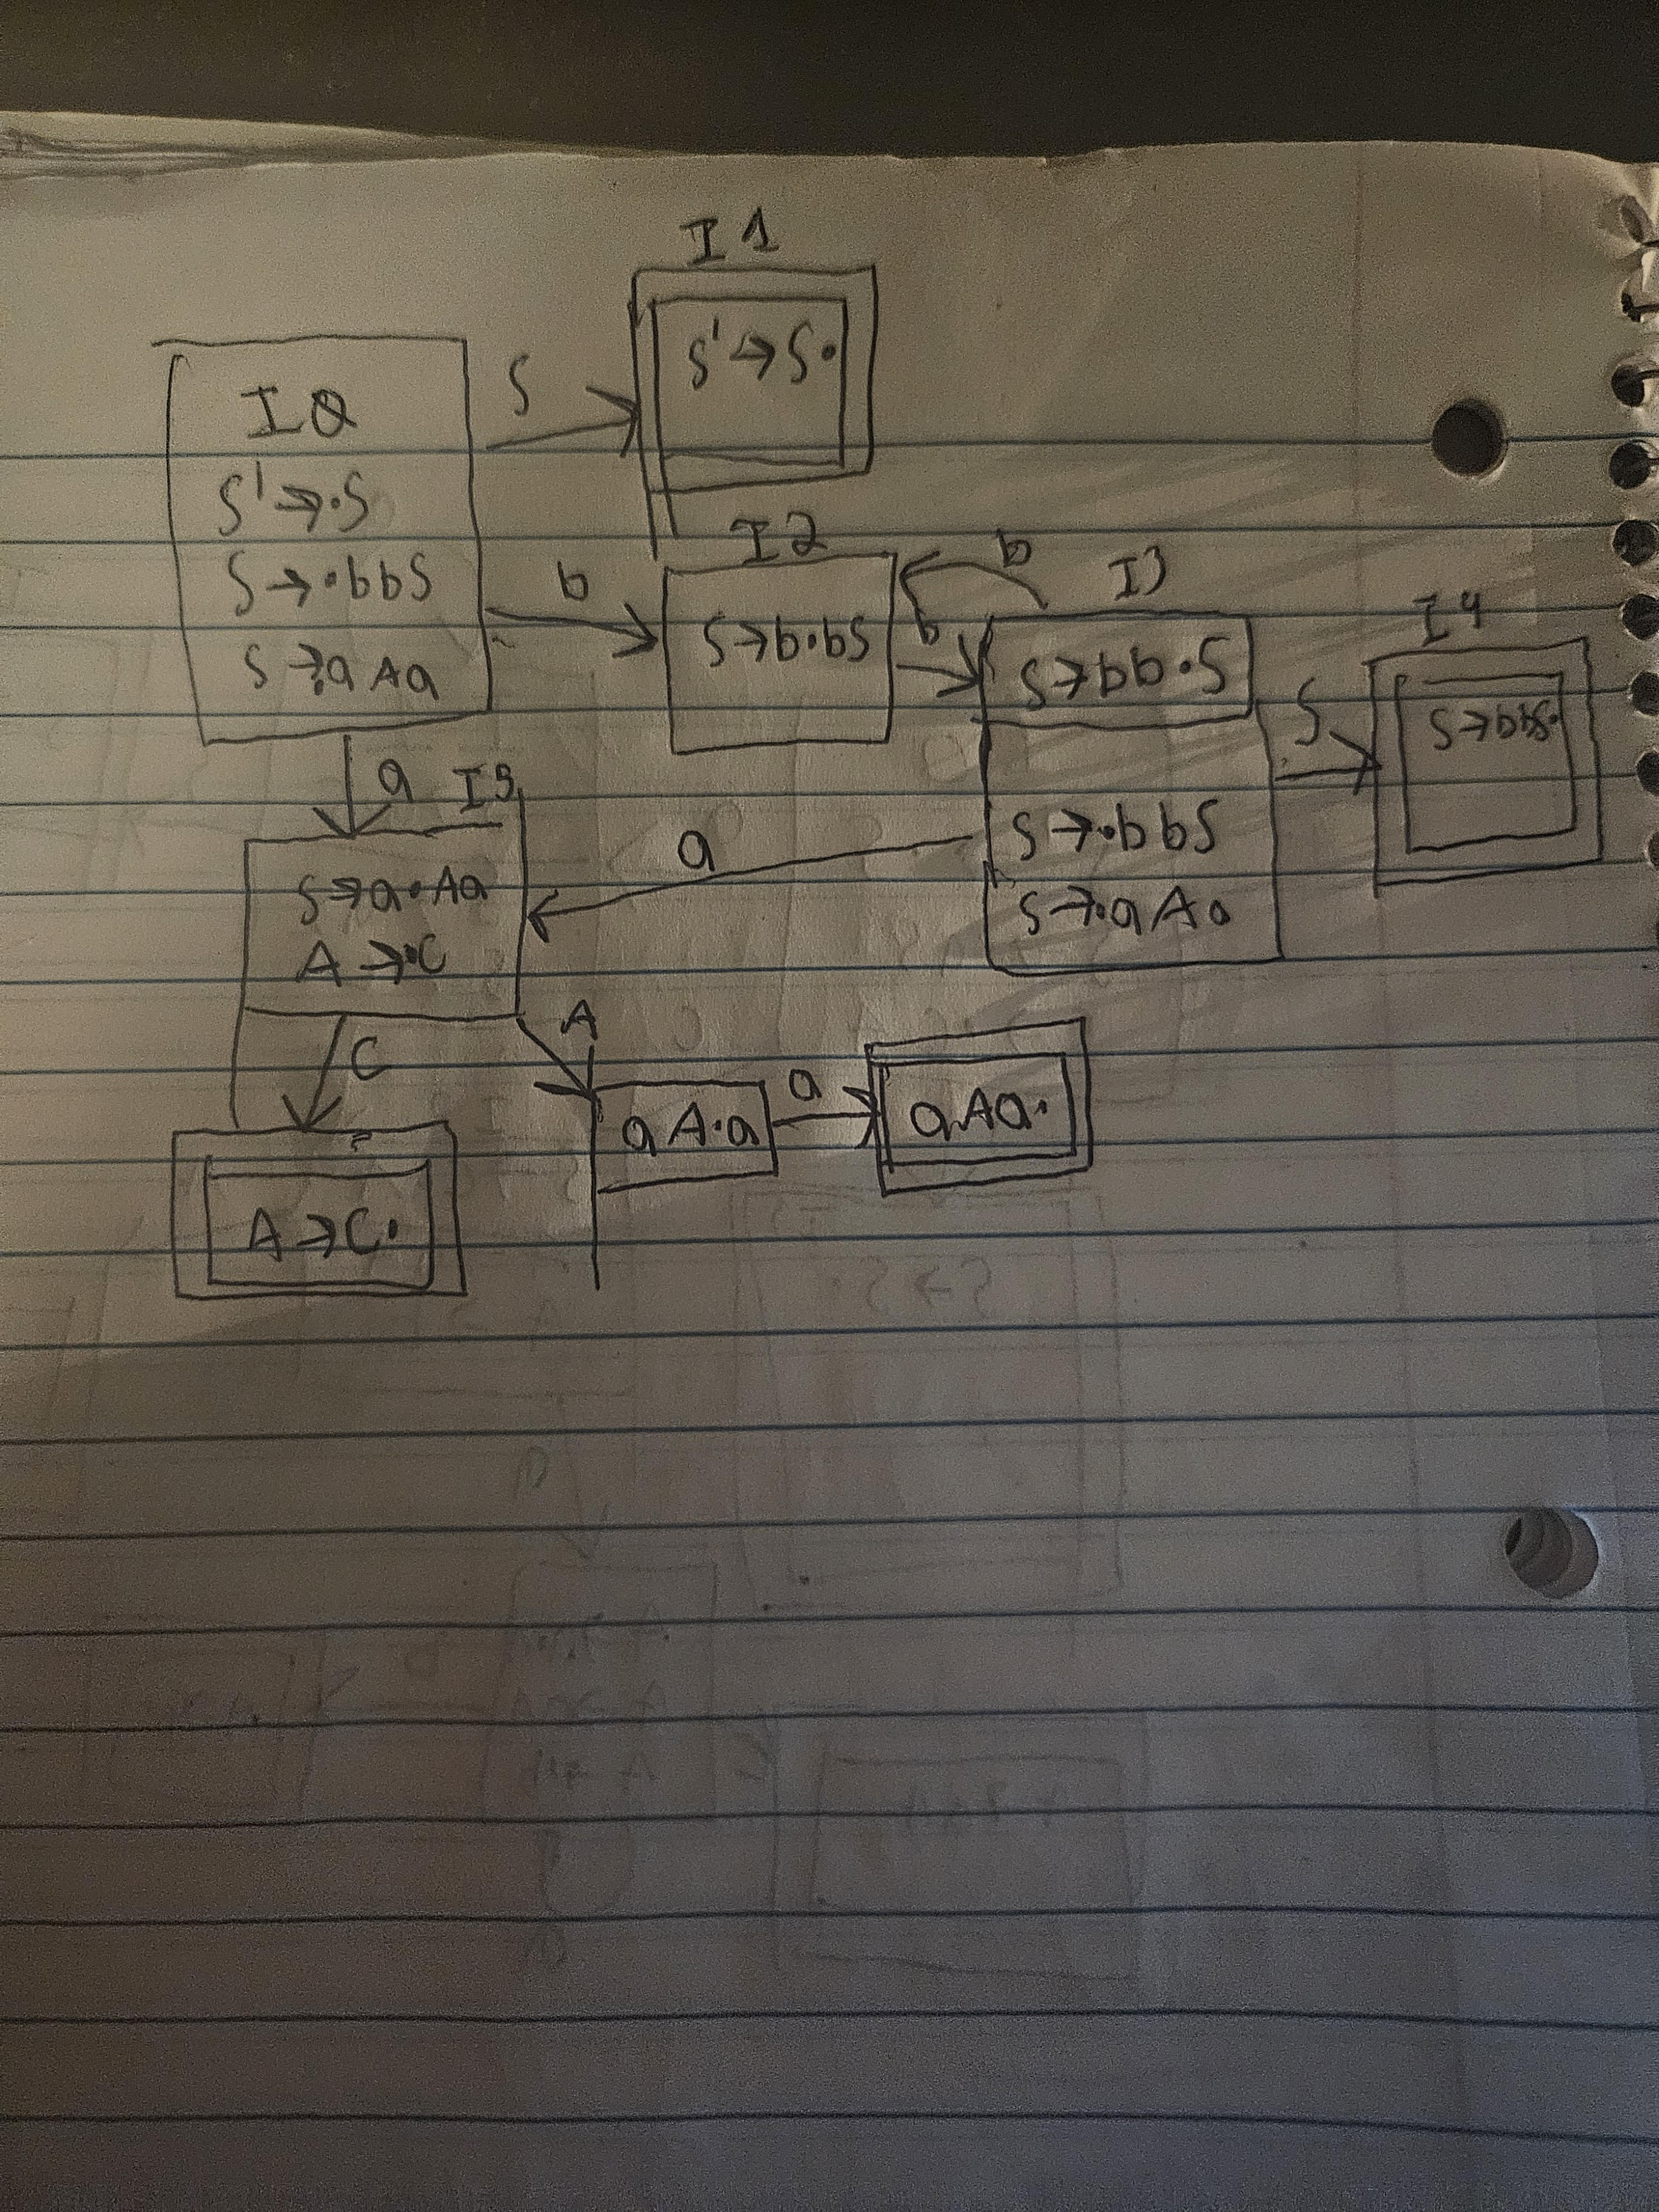
\includegraphics[width=0.5\textwidth, angle=0]{figures/DFA3.jpg}
	\end{center}
    \end{enumerate}
    \newpage
    \section*{Question 5}
    \begin{enumerate}
	\item Give the initial item set
		\[S' \rightarrow S\]
		\[S \rightarrow BCa\]
		\[ B \rightarrow bB\]
		\[ B \rightarrow cC\]
	\item How many Initial Outgoing states are there and What are there labels
	There exists 4 labels that are coming out of S' they are S, B, b, c
	\item Give complete DFA Diagram
	\begin{center}
            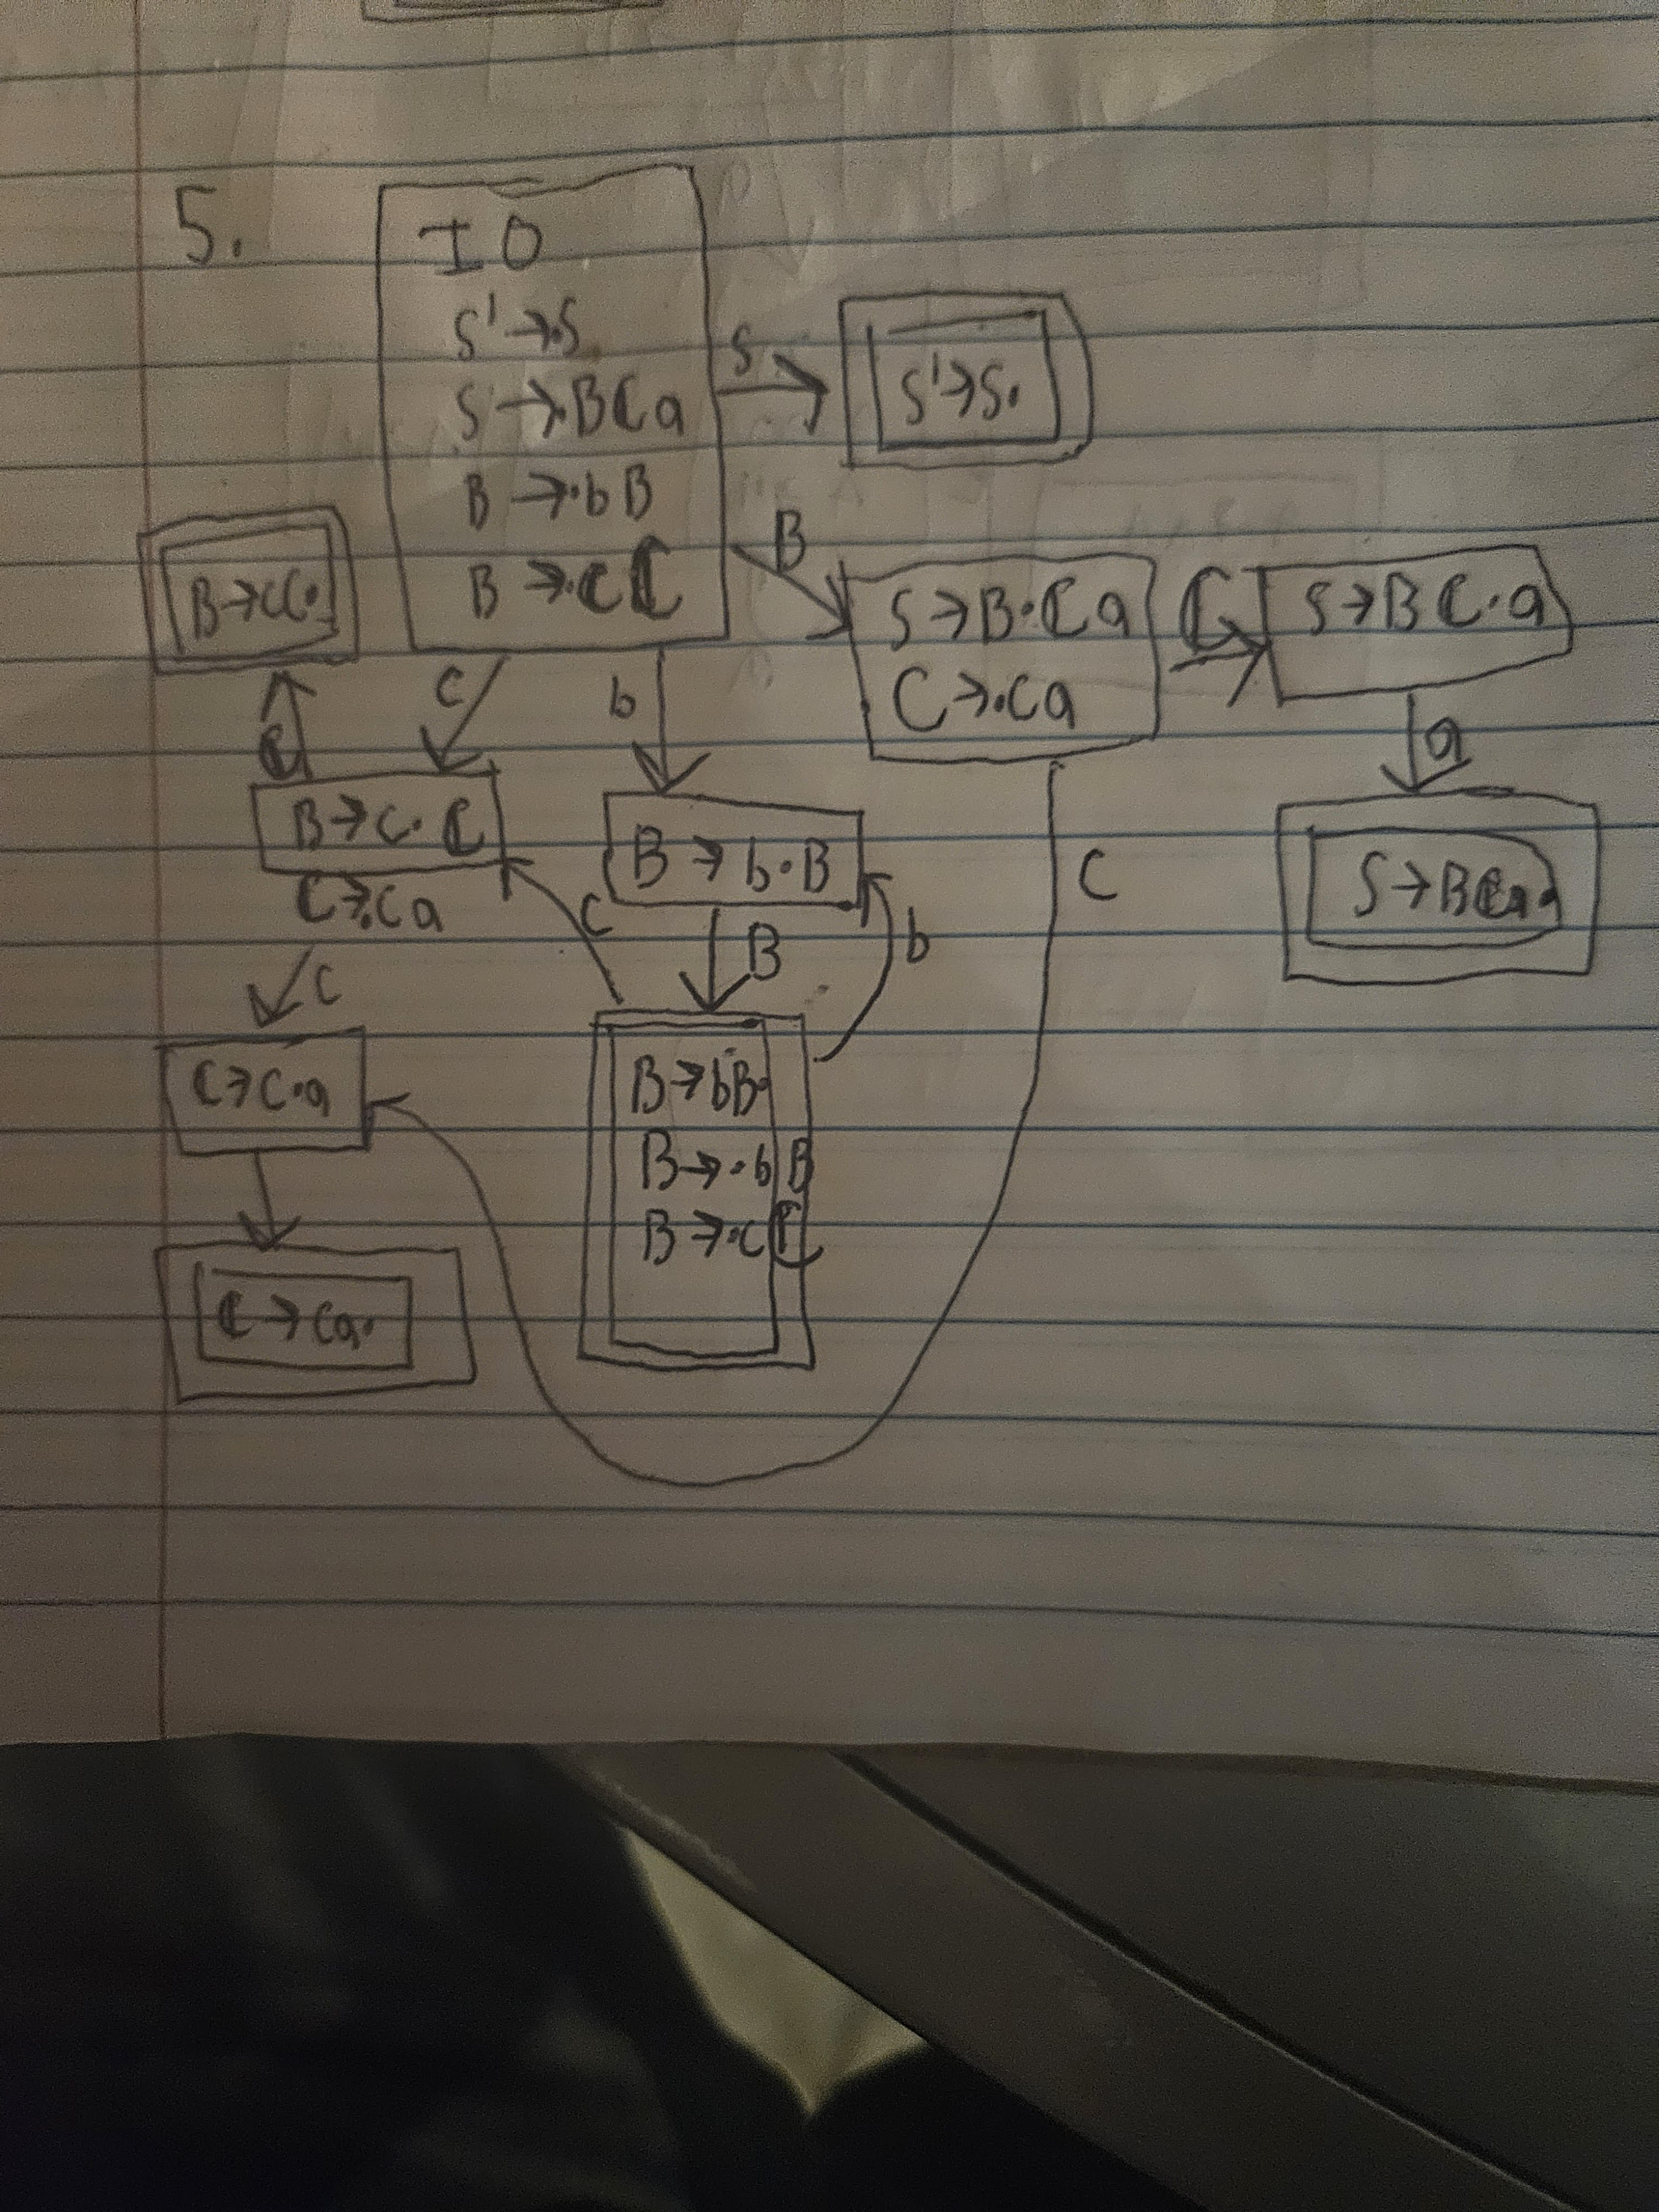
\includegraphics[width=0.5\textwidth, angle=0]{figures/DFA4.jpg}
	\end{center}
    \end{enumerate}
    \section*{Question 6}
    \begin{enumerate}
	\item Give the list of actions for each step for graph 1
		\[(S, a),(S, b),(S, b2),(R, b \rightarrow A),(S, c),(R, (c, A) \rightarrow S),(R, (S, a, b) \rightarrow S),ACC\]
	\item Give the list of actions for each step for graph 2
		\[(S, a),(S, b), (S, b), (R, (b \rightarrow A)), (S, c),  (R, (c, a))\rightarrow S, (R, (S,b,a) \rightarrow S),ACC\]

    \end{enumerate}
    \section*{Question 7}
    \begin{enumerate}
	\item Which possible states could you be in assuming you reduced $q_4$? Give the path's that reached that state?
	The following states are possible
		    \[\left\{ q_3, q_5 \right\}\]
	The List of possible paths would be
		\[q_0 \rightarrow q_2 \rightarrow q_3 \rightarrow q_6\]
		\[q_0 \rightarrow q_2 \rightarrow q_3 \rightarrow q_5 \rightarrow q_6\]
	\item Suppose you have reached $q_4$ and reduced $A \rightarrow b$ Which states could you be in and which paths reach that state?
	The only possible state that I could be in is
		\[ \left\{ q_3 \right\}\]
	And the only path to reach $q_3$ is
		\[ \left\{ q_0 \rightarrow q_2 \rightarrow q_3 \rightarrow q_4 \right\}\]
	\item Suppose you have reached $q_7$ and reduced $A \rightarrow aA$ Which states could you be in and which paths reach that state?
		We know that I must be in the state
		    \[\left\{ q_5 \right\}\]
		The only paths to reach $q_7$ is
		\[q_0 \rightarrow q_2 \rightarrow q_3 \rightarrow q_5 \rightarrow q_7 \]
		it is worth noting that $q_5$ can be infinitely looped to by itself
	\newpage
	\item trace the acceptance for string $ccab$
        \begin{center}
            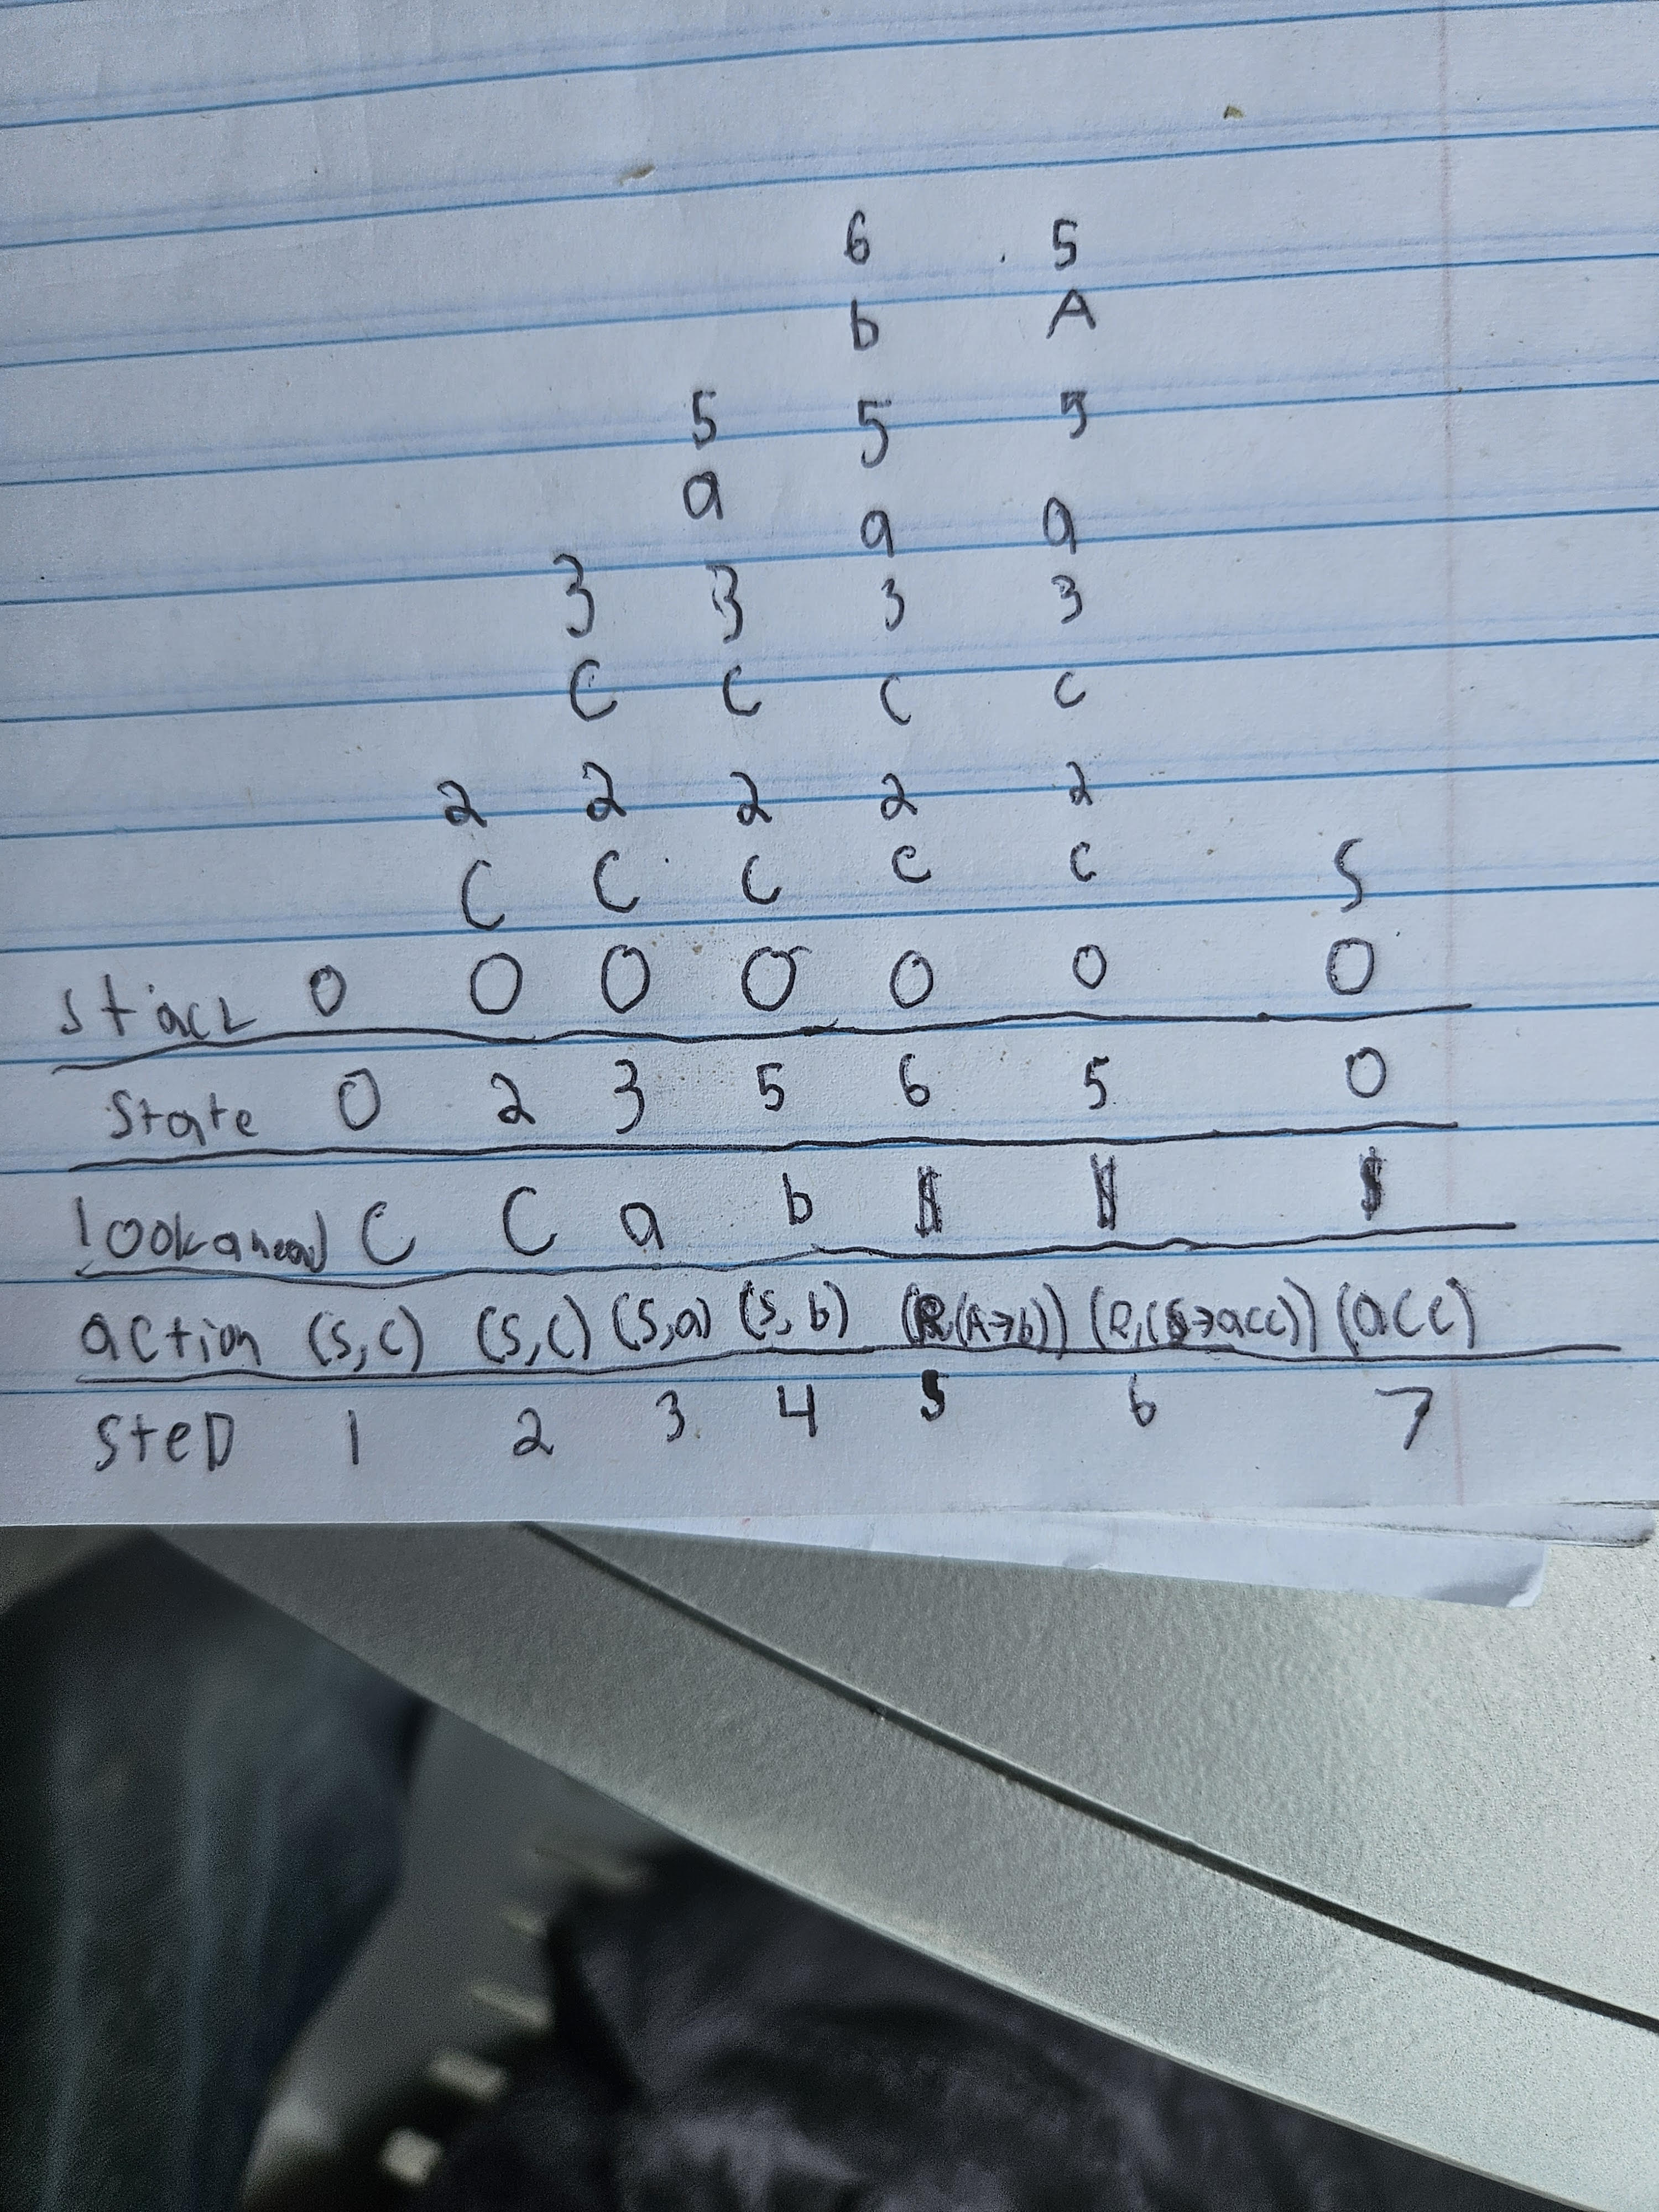
\includegraphics[width=0.5\textwidth, angle=0]{figures/DFA5.jpg}
        \end{center}

    \end{enumerate}
\end{document}
